% This is samplepaper.tex, a sample chapter demonstrating the
% LLNCS macro package for Springer Computer Science proceedings;
% Version 2.20 of 2017/10/04
%

\documentclass[runningheads]{llncs}
%
\usepackage{graphicx}
\usepackage[noend]{algpseudocode}
\usepackage{algorithmicx,algorithm}
\usepackage{subfigure}
\usepackage{cite}
\usepackage{amsmath}
\usepackage{multirow}
\usepackage{geometry}
\usepackage{booktabs}
% Used for displaying a sample figure. If possible, figure files should
% be included in EPS format.
%
% If you use the hyperref package, please uncomment the following line
% to display URLs in blue roman font according to Springer's eBook style:
% \renewcommand\UrlFont{\color{blue}\rmfamily}

\begin{document}
%
\title{MC-ODG:Multi-category oversampling based on DBSCAN and Gaussian distribution\thanks{Supported by organization x.}}
%
%\titlerunning{Abbreviated paper title}
% If the paper title is too long for the running head, you can set
% an abbreviated paper title here
%
\author{First Author\inst{1}\orcidID{0000-1111-2222-3333} \and
Second Author\inst{2,3}\orcidID{1111-2222-3333-4444} \and
Third Author\inst{3}\orcidID{2222--3333-4444-5555}}
%
\authorrunning{F. Author et al.}
% First names are abbreviated in the running head.
% If there are more than two authors, 'et al.' is used.
%
\institute{Princeton University, Princeton NJ 08544, USA \and
Springer Heidelberg, Tiergartenstr. 17, 69121 Heidelberg, Germany
\email{lncs@springer.com}\\
\url{http://www.springer.com/gp/computer-science/lncs} \and
ABC Institute, Rupert-Karls-University Heidelberg, Heidelberg, Germany\\
\email{\{abc,lncs\}@uni-heidelberg.de}}
%
\maketitle              % typeset the header of the contribution
%
\begin{abstract}
%The abstract should briefly summarize the contents of the paper in
%15--250 words.
Classification on imbalanced data is one of the most
challenging classification tasks in machine learning. 
In the predicting task,
the imbalanced distribution of data leads 
to the poor prediction ability for minority classes.
According to the number of different classes, the classification problem 
can be divided into binary classification problems and multiclassification problems. Due to 
the complex relationship between different classes,
the difficulity of multi-class problems on imbalance data 
is much greater. Many scholars have proposed disirable oversampling methods to
solve the problem of classification on imbalance data, such as SMOTE and its derivatives.
But these methods are easily affected by noise and 
overlapping data distributions, and cannot handle clusters form data.
Therefore we propose new oversampling methods called ODG and MC-ODG, In these methods,
DBSCAN and gaussian distribution were applied to generate new sample points. The experiment results
show that our methods has high prediction ability compared to state-of-art methods.

\keywords{imbalance data \and oversampling \and DBSCAN \and Gaussian distribution.}
\end{abstract}
%
%
%
\section{Introduction}
%指出什么是不平衡数据集
Imbalanced data\cite{2004Editorial} refers to data sets that have an uneven 
amount of data between different classes. In the binary classification problem, 
we assume that the majority class are negative class and 
the minority class are positive class.
%不平衡数据处理的重要性,现在典型方法中存在的问题
The actual demand shows the importance and difficulty of learning on imbalanced data distributions.
The imbalance occurs in many fields, such as medical 
diagnosis\cite{2013Computational,2019Electrocardiogram} and fault detection\cite{2018Imbalanced}.
disease samples in medical diagnosis and fault samples in fault detection are minority samples.
Although the sample size of minority class is small, 
we tend to be interested in minority samples because minority samples tend to contain more value.
The disease samples need to be predicted more accurately than the normal samples, 
and the cost of misjudging fault samples is much higher than misjudging normal samples.
The difficulty in solving imbalanced data sets lies in the fact that existing machine 
learning models tend to skew the prediction results towards 
majority class in the process of prediction\cite{Victoria2013An}, then 
the minority class cannot be classified correctly\cite{2016A}. 
Therefore, More advanced algorithms need to be proposed to better prediction of minority samples.

%现有的处理不平衡数据集的方法
The methods dealing with imbalanced data sets can be roughly
divided into two types: algorithm-level\cite{Myoung2015Geometric} and data-level\cite{2002SMOTE}.
Algorithm-based approaches include BalanceCascade\cite{2019Class}, Adaboost\cite{10.1007/3-540-59119-2_166}, 
XGBoost\cite{Chen_2016}, and more. But algorithm-based methods are limited 
to a single type of classifier\cite{2020Combined} and cannot be extended to more general machine learning models.
The data-level methods perform data preprocessing with the aim of reducing the imbalance ratio. Therefore 
the data can be processed by general machine learning models.
Data-level methods are generally divided into undersampling\cite{2015Undersampled} 
and oversampling\cite{2002SMOTE}. undersampling decrease the number of majority samples,the price is losing part of the information, 
while oversampling enhances minority class by introducing new samples\cite{2010A}. 
In our work, oversampling is used to preprocess the data.

%介绍基于数据的smote方法

Data-level methods address the imbalance by changing the data distributions and can be 
applied with general mechine learning methods.
SMOTE is an improved method based on the random oversampling algorithm, 
which realizes 
oversampling by randomly generating new sample points 
on the line of minority sample points.
Numerous modifications of SMOTE algorithm have been proposed in the literature, such as
Borderline-SMOTE\cite{2005Borderline}, ADASYN\cite{2008ADASYN}. SMOTE and its derivatives have their weaknesses,
Methods based on SMOTE are susceptible to noise points and are difficult to deal with overlapping.
The generated minority points and majority points are covered, 
which affects the separating hyperplane of the classifier. In addition, $SMOTE$ method is also poor in the process
of cluster data. SMOTE is unable to capture the cluster distributions
if the monority sample points are distributed in clusters.
Furthermore,
the method of syntheticing new points by SMOTE is relatively single,
so the generated data points are difficult to maintain the 
original data distributions\cite{2008DATA}.
After using $SMOTE$ to generate new data, 
the data distributions of minority sample points may change, which will affect the prediction progress.


 %二分类和多分类
 SMOTE and its derivatives are less effective when dealing with multiple classification problems 
 \cite{2020Combined,2011LIBSVM}.The relationship between two classes is relatively simple,
but in multi-classification problems, the relationship between classes becomes much more complex\cite{2017Relevance}.
Especially when dealing with sample points near the multiple category boundaries, 
Create overlapping data distributions\cite{Jierui2013Overlapping} is hard to avoid.
The existing methods dealing with multi-classification include transforming 
the multi-classification problem into binary classification problems(OVO)\cite{articlemulti}, 
But processing two classes separately will ignore the rest classes' information.
Multiple classification problems can also be divided into one-to-many problems(OVA) instead,
Treat one class as a minority class and the rest as a majority class.
However, this does not capture the relationships between majority classes effectively.
New approach should to be adaptive to multi-classification problems.

%给出聚类算法
If minority sample points are distributed in clusters, we could use cluster methods.
Clustering algorithm\cite{2011Data,inproceedings} divides the same set of data into multiple sets, 
and the data in each set is similar. We can use the clustering algorithm 
to divide the data into multiple clusters and oversample data in each cluster. There are many kinds of clustering algorithms, 
among which the most famous one is K-MEANS\cite{2007K} algorithm.
However, K-MEANS algorithm is a distance-based algorithm. 
When there are irregular clusters, K-MEANS algorithm is difficult to handle, 
meanwhile the parameter K is difficult to set. Therefore, 
We use DBSCAN\cite{2013Mining} algorithm based on density.


%提出新的方法
Our work is to propose a new oversampling method.
The above mentioned methods is sensitive to noise, 
easy to produce overlapping and unable to deal effectively with cluster distribution data.
To solve these problems, 
we proposed ODG and MC-ODG algorithms.
The proposed algorithm can solve the above problems 
while the new sample points can retain the original data distributions.
The ODG algorithm can be adaptive to determine how to 
generate new sample points and how many sample points are generated around what kinds of points.
The new algorithms apply DBSCAN clustering method and Gaussian
 distributions\cite{SEEGER2004GAUSSIAN} to fit the data.
 The experiments resuls show that
 the proposed algorithms are superior to the existing oversampling 
 methods on different metrics.

%总结贡献
To summarize, our work makes the following contributions.
\begin{itemize}
  \item ODG is an oversampling method that can effectively process clustered data.
  \item We explain the influence of noise data points on the oversampling process 
  and ODG shows how to deal with noise data points.
  \item ODG preserves the original data distributions after oversampling.
  \item ODG is suitable for binary classification, and its extension MC-ODG is suitable for multi-classification problems.
\end{itemize}

%文章组织
The paper is organized as follows.The next section introduces 
the knowledge required for our ODG and MC-ODG algorithms, 
as well as the existing oversampling methods. Section 3 introduces our ODG and MC-ODG 
algorithms in details, 
and gives the specific flow of the algorithms and the corresponding complexity analysis.
In section 4, we introduce a series 
of comparative experiments based on different models, 
and the analysis and results of the experiments
are given. Section 5 gives the summary and our future works.


\section{Related work}
In this section,
 we propose the required knowledge and some related over-sampling methods dealing with imbalanced data.
\subsection{Clustering method}
Clustering algorithm is to find groups of similar data, and each group of similar data forms a cluster\cite{inproceedings}.
 There may be multiple clusters in a single minority class data, 
we need to use clustering algorithm to identify multiple clusters
 and then process each of them.
The most famous clustering methods include distance-based K-MEANS algorithm and density-based DBSCAN algorithm.
K-MEANS algorithm is relatively easy, but the algorithm must determine the number of clusters K.
Meanwhile, compared with density-based DBSCAN algorithm, K-MEANS cannot find clusters with various shapes.
DBSCAN defines a cluster as the largest set of points
 connected by density and can find clusters of arbitrary shape. After the whole process, the algorithm classifies the sample points into core points,
  borderline points and noise points.
 Given the parameters $eps$ and $min\_pts$, we will get three kinds of points. Core points have no less than
  $min\_pts$ points in the $eps$ neighborhood. Borderline points refer to that were partitioned into a cluster after DBSCAN,
  but not belong to core points. After the DBSCAN algorithm, The points were not divided into any cluster defined as noise points.
The core points can best represent the distribution of the corresponding cluster.

\subsection{Algorithm-level methods}
Algorithm-level methods are based on proposing 
new models to solve the problem of imbalanced data prediction\cite{Chen_2016,2007LogitBoost}.
 Algorithm-level methods can be broadly divided into cost-sensitive 
 methods\cite{2010Risk} and ensemble methods\cite{2003SMOTEBoost}.
The cost-sensitive methods change the weights or loses to improve the performance of classifier, such as 
adaboost\cite{10.1007/3-540-59119-2_166}, which is a lifting algorithm,
and the weights of the minority samples misclassfied will gradually increase.
Ensemble classifier improves the learning result by combining
 a group of basic classifiers together.
 The classification of ensemble methods are Boosting\cite{article_boosting} and Bagging\cite{2018Multi}.
 Boosting methods include SMOTEBoost\cite{2003SMOTEBoost},
XGBoost\cite{Chen_2016}, LogitBoost\cite{2007LogitBoost}, and so on.
Although some algorithm-level approaches have good classification ability, 
algorithm-level methods are limited to single-type classifiers\cite{2020Combined}.
This kind of solutions cannot be extended to more general machine learning models.

\subsection{Data-level methods}
unsersampling methods \cite{2004Editorial,2004Minority} remove majority points 
so as to make the data balanced. Famous undersampling methods include random undersampling\cite{2018Imbalanced}, 
$EasyEnsemble$\cite{2020EASY} and $NearMiss$\cite{2011Data}.
$BalanceCascade$\cite{2019Class} mentioned earlier also adopts the idea of undersampling.
But some information will be lost when majority points are discarded by undersampling.
Oversampling, on the other hand, balances the distribution of data by generating new data points without losing information.

The fundamental idea of SMOTE is to generate new sample by interpolation between minority class samples\cite{2018SMOTE}.
Specifically, for a certain sample $x_i$, one of the K nearest neighbors is randomly selected as $x_i ^{'}$.
Use the equation\ref{equation14} to generate a new sample $x_{new}$. $\epsilon \in [0,1]$ is a random number.
\begin{equation}
  \label{equation14}
  x_{new}=x_i+(x_i-x_i^{'})\times \epsilon
\end{equation}
We can easily find the weakness of SMOTE,
Using the algorithm of SMOTE, Generating new sample points inside the minority sample points is easy, 
but new points are far from the classification surface, which has little influence on the classification prediction.
SMOTE algorithm is easily affected by noise, 
the new synthetic samples may overlap with majority class samples.
Borderline-SMOTE\cite{2005Borderline} is based on SMOTE, this algorithm classifies
the minority points into three types, 
$noise$, $danger$ and $safe$.
All the K nearest neighbor samples of the $noise$ class are majority points, 
more than half of the K nearest neighbor samples
of the $danger$ points are majority points, and all of K nearest neighbor samples of $safe$ points are minority points.
Borderline-SMOTE uses $danger$ points to generate new points.
To a certain extent Borderline-SMOTE reduced the negative effect of noise and overlapping data distribution.
ADASYN\cite{2008ADASYN} is an adaptive composite sampling method, 
a mechanism is used to determine how many samples need to be synthesized for each minority sample point.
In general, for a minority sample point, more majority sample points in its K nearest neighbors, 
the more minority class sample points will be generated near this point.
There are also methods conbined oversampling and undersampling, such as SMOTE+ENN\cite{2019Electrocardiogram},
This method first deleted majority points ,of which all of K nearest neighbors are minority points.
Then use SMOTE to generate new samples.

The way of generating new data in SMOTE is too simple, 
Simply generating data on the line does not effectively preserve the original data distribution\cite{2017CCR,2020Combined}.
In addition, for the problem of multiple classification, 
methods based on SMOTE could not make use of the relationship between multiple classes during the process of 
generation and expected effect cannot be achieved.
$CCR$ and MC-CCR algorithms are oversampling methods based on $energy$,
In these methods, a spherical region is drawn at the center of each sample point of a minority class. 
The spherical region is constantly expanding, when meeting a majority point the energy is reduced.
When the $energy$ is exhausted, the region will no longer extend.
New data points are randomly generated inside the spherical region. 
The number of generated data is inversely proportional to the radius of the spherical region.
In addition, this method also proposed $cleaning$ process, 
the majority points inside the spherical area will be shifted out to reduce overlapping.
But the CCR approach also has its drawbacks. In the process of generating data points,
the CCR method generates data randomly in the region without considering the distribution of data points.
In addition, the CCR method may synthetic too many sample points near the noise points. 
As the radius of the spherical region corresponding 
to a noise point is small, many sample points will be generated, which may affect the prediction results.
However, the proposed algorithm can identify the noise of minority points and 
avoid generating data around the noise.

\begin{algorithm}[htbp]
  \caption{ODG} %算法的名字
  \label{alg1}
  \hspace*{0.02in} {\bf Input:} %算法的输入, \hspace*{0.02in}用来控制位置,同时利用 \\ 进行换行
   \\$M$ $\leftarrow$ majority points  \\
   $m$ $\leftarrow$ minority points  \\
   $N_{maj}$ $\leftarrow$ number of sample points for majority class  \\
   $N_{min}$ $\leftarrow$ number of sample points for minority class  \\
   $\alpha_{borderline}$ $\leftarrow$ the ratio of samples generated by borderline samples\\
   $noise\_ratio$ $\leftarrow$  ratio threshold of noise sample points  \\
   $eps$ $\leftarrow$ the parameters of DBSCAN \\
   $min\_pts$ $\leftarrow$ the parameters of DBSCAN \\
   
  \hspace*{0.02in} {\bf Output:} %算法的结果输出
  Minority points and Majority points

  \begin{algorithmic}[1]
  \State $m_{core}$,$m_{borderline}$,$m_{noise}$=DBSCAN(m,$eps$,$min\_pts$) % \State 后写一般语句
  \State $N_{oversampling}$=$N_{maj}$-$N_{min}$
  \If{$len(m_{noise})/N_{min}<noise\_ratio$}
      \State $N_{noise}$=0
  \Else
      \State ratio=$len(m_{noise})/N_{min}<noise\_ratio$ 
      \State $\alpha_{noise}=\frac{0.9}{1-{noise\_{ratio}}^2}\times ratio^2+1-\frac{0.9}{1-{noise\_ratio}^2}$
      \State $N_{noise}=\alpha_{noise} \times N_{oversampling}$
      \State $N_{noise}=min(multiple\_k \times K \times len(m_{noise}), N_{noise})$
  \EndIf
  \State $N_{oversampling}$=$N_{oversampling}$-$N_{noise}$
  \State $N_{borderline}$=$N_{oversampling} \times \alpha_{borderline}$
  \State $N_{core}$=$N_{oversampling}$-$N_{borderline}$
  \State clusters $\leftarrow$ clustering of minority points
  \State $cov\_mats$ $\leftarrow$ Calculate the variance of the core points of each cluster,scale according to the number of core points
  \State $new\_data$ $\leftarrow$ an empty set.
  \State $translations$ $\leftarrow$ a zero matrix, the same shape as $M$.
  \State $generate\_borderline(m_{boaderline},N_{borderline},translations,core\_points,new\_data,cov\_mats,$multiple\_k$)$
  \State $generate\_core(clusters,N_{core},new\_data)$
  \State $generate\_noise(N_{noise},m_{noise},$new\_data$)$
  \State $M$ $\leftarrow$ $M+translations$
  \State $m$ $\leftarrow$ $m$ concatenate with $new\_data$
  \State \Return $M$,$m$
  \end{algorithmic}
  \end{algorithm}

\section{ODG Algorithm and MC-ODG Algorithm}
In this section we will introduce ODG algorithm and MC-ODG algorithm.
The methods based on SMOTE are not able to effectively deal with noise points and cluster distribution data.
The noise in the data will lead to overlapping data distributions after oversampling.
Also, the data point generated by SMOTE cannot preserve the original distributions.
MC-CCR randomly generates points in 
a certain range without retaining the original distributions of a minority points.
Furthermore, this method may generate too many samples of 
minority points near the noise, which will adversely affect the prediction results.
Aiming at the shortcomings of the above methods, 
we propose ODG and MC-ODG to avoid the problems mentioned above.

\subsection{Binary inbalanced classification}
We first give the ODG algorithm, which is used to solve the binary classification problems.
The whole ODG algorithm process can be roughly divided into clustering 
minority sample points and generating new samples near borderline points, core points and noise points respectively.
The flow of ODG is shown in the algorithm \ref{alg1}.
\subsubsection{Clustering}
We cluster the minority sample points firstly.
\begin{figure}[htbp]
  \centering
  \subfigure[$K-means$]{
  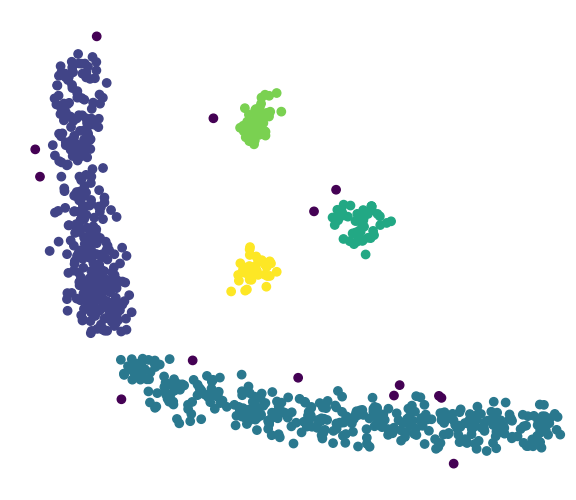
\includegraphics[width=.3\textwidth]{myplot5_1.png}
  %\caption{fig1}
  }
  \quad
  \subfigure[$DBSCAN$]{
  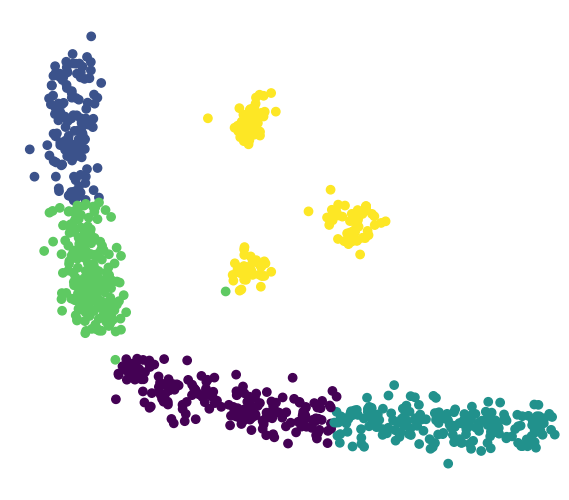
\includegraphics[width=.3\textwidth]{myplot5_2.png}
  }
  \caption{The comparision of $K-means$ and $DBSCAN$}
  \label{fig19}
  \end{figure}
The results of K-MEANS and DBSCAN are shown in figure\ref{fig19}.
The same color represents the same cluster.
Obviously, the result of DBSCAN is more consistent with the data distribution.
Therefore we use DBSCAN as the clustering method. 
After DBSCAN, 
the minority sample points are divided into core points, borderline points and noise points.
Next, we need to generate new points around different kinds of points respectively.
We assume that the number of majority sample points is $N_{maj}$,
and the number of minority sample points is $N_{min}$, then the number of oversample points $N_{oversampling}$ is shown 
as equation \ref{equation1}.
\begin{equation}
  \label{equation1}
  N_{oversampling}=N_{maj}-N_{min}
\end{equation}
After obtaining the total number of oversampled samples, 
we need to determine the proportion of generated sample points near the core points, borderline points and noise points.
Sample points should not be generated 
near the noise unless it is impossible to form effective clusters on minority points.
The failure to form clusters means that most of the sample points are marked as noise points after the DBSCAN algorithm
, which we will deal with specially.
In general, $N_{noise}$ is zero. we note the ratio of generated new sample points 
at borderline points is $\alpha_{borderline}$,
Then the number of generated samples $N_{borderline}$ and $N_{core}$ are shown in equation \ref{equation2}.


\begin{equation}
  \label{equation2}
\begin{aligned}
  & N_{borderline}=N_{oversampling}\times \alpha_{borderline} \\
  & N_{core}=N_{oversampling}-N_{borderline}
\end{aligned}
\end{equation}

\begin{figure}[htbp]
  \centering
  \subfigure[$\alpha_{borderline}$]{
  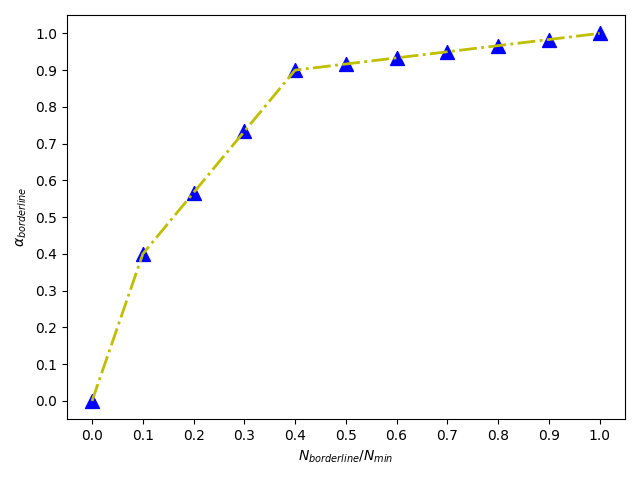
\includegraphics[width=.3\textwidth]{myplot10.png}
  %\caption{fig1}
  }
  \quad
  \subfigure[$\alpha_{noise}$]{
  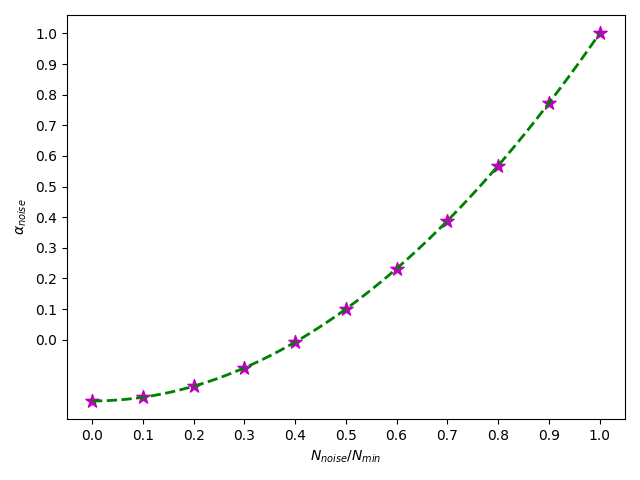
\includegraphics[width=.3\textwidth]{myplot11.png}
  }
  \caption{}
  \label{fig20}
  \end{figure}

The parameter $\alpha_{borderline}$ can be specified as a 
hyperparameter and can be adaptive based on the ratio of borderline points.
In general, $\alpha_{borderline}$ is greater than the ratio of the boundary points,
because we prefer to generate data near borderline points,
then the classification surface is biased to minority points.
Figure \ref{fig20}(a) shows the relation with $\alpha_{borderline}$ and $\frac{N_{borderline}}{N_{min}}$


\subsubsection{Generate data near borderline points}
\begin{algorithm}[htbp]
  \caption{$generate\_borderline$}
  \label{alg3}
  \hspace*{0.02in} {\bf Input:} %算法的输入, \hspace*{0.02in}用来控制位置,同时利用 \\ 进行换行
   $m_{borderline}$,$N_{borderline}$,$translations$,$core\_points$,$new\_data$
   $cov\_mats$,$multiple_k$
  \begin{algorithmic}
    \For{point in $m_{borderline}$} % For 语句,需要和EndFor对应
      \State Calculate K nearest neighbors of point.
      \State $cov\_mat$ $\leftarrow$ Find the covariance matrix corresponding to the point from $cov\_mats$
      \State $d\_max$ $\leftarrow$ maximum distance of knearest neighbors.
     \State $n_{borderline}=min(\frac{n\_knearest\_maj}{\sum_{i\in minority} n\_knearest\_maj}\times N_{boardline},multiple\_k \times K)$
      \State $tem\_data=multivariate\_normal(mean(core\_points),cov\_mat,n_{borderline})$
      \State add $tem\_data$ to $new\_data$.
      \For{for $m_{j}$ in $k\_nearest\_maj$}
        \State $translations_j$=$translations_j$+$\frac{d_{max}-d_{j}}{d_{j}}\times (m_{j}-point)$
      \EndFor
  \EndFor
  \end{algorithmic}
\end{algorithm}
In order to make the distribution of the generated new sample points consistent with the core
points corresponding to the borderline point, gaussian distribution is adopted.
We first need to determine $n_{boardline}$ for a particular borderline point.
We calculate the K nearest neighbors of each borderline point. 
If the K nearest neighbor of the minority point have more majority sample points, means the point 
is closer to the decision boundary, and more sample points should be generated near this point.
We set the number of majority sample points is $n\_knearest\_maj$,
then $n_{boardline}$ can be obtained in equation \ref{equation4}.
\begin{equation}
  \label{equation4}
  n=\frac{n\_knearest\_maj}{\sum_{i\in minority} n\_knearest\_maj}\times N_{boardline}
\end{equation}
We need to limit the maximum value of $n_{boardline}$
to avoid generating too many minority samples around one single point because
extreme distribution may exist in some of datasets. If too many points are generated near one sample point.
the original data distribution is changed and the training of the model is adversely affected.
Therefore we limit the value of $n_{boardline}$ . We define the parameter $multiple\_k$,
Limit the maximum of $n_{borderline}$ to $multiple\_k\times K $, as shown in equation\ref{equation5}.
\begin{equation}
  \label{equation5}
  n_{boardline}=min(multiple\_k \times k, n_{boaderline})
\end{equation}
\begin{figure}[htbp]
  \centering
  \subfigure[]{
  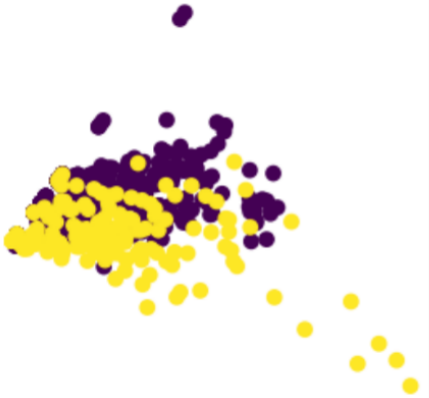
\includegraphics[width=.25\textwidth]{myplot2_1.png}
  %\caption{fig1}
  }
  \quad
  \subfigure[]{
  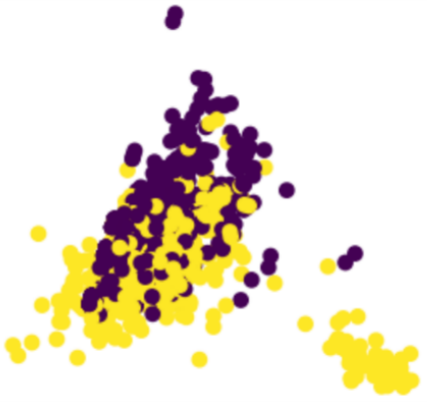
\includegraphics[width=.25\textwidth]{myplot2_2.png}
  }
  \quad
  \subfigure[]{
  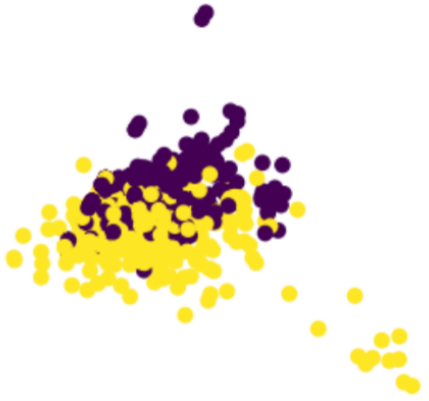
\includegraphics[width=.25\textwidth]{myplot2_3.png}
  }
  \caption{
    (a)is initial dataset,(b) and (c) are oversampling results, (c) has limited the number of generation.}
  \label{fig15}
  \end{figure}

In Figure\ref{fig15},(a) is initial dataset,
(b) is the data distribution obtained without limiting the number of individual sample points generated,
(c) limited the number of generation.
We can find that too many sample points are generated near one sample point in the lower right of Figure\ref{fig15}(b)
, thus affecting the overall distribution of minority points. 
Obviously Figure\ref{fig15}(c) is more consistent with the distribution of the original data.

After clustering, each borderline point corresponds to a certain cluster, 
and the core points of this cluster can best represent the distribution of this cluster.
We calculate the covariance matrix corresponding to the core points, 
then use gaussian distribution to generate sample points at the corresponding borderline points after scaling it.
We set the particular borderline point is $point$, $cov$ is the function to calculate the covariance matrix,
and the number of core points is $num\_core\_points$,
The function to generate a new sample point using gaussian distribution is $multivariate\_normal$,
New sample points $new\_data$ can be obtained by equation\ref{equation3}.
\begin{equation}
  \label{equation3}
  \begin{aligned}
     & cov\_mat=cov(core\_points)/num\_core\_points \\
     & new\_data=multivariate\_normal(point,cov\_mat,n_{boardline})
  \end{aligned}
\end{equation}
The algorithm for generating new sample points at borderline points is algorithm\ref{alg3}.

\subsubsection{Generate data near core points}
\begin{algorithm}[htbp]
  \caption{$generate\_core$}
  \label{alg4}
  \hspace*{0.02in} {\bf Input:} $clusters$,$N_{core}$,$new\_data$
  \begin{algorithmic}
    \For{cluster in clusters}
    \State $n_{core}=\frac{num\_data\_cluster}{\sum_{i \in cluster} num\_data\_cluster} \times N_{core}$
    \State $core\_points$ $\leftarrow$ core of cluster
    \State $cov\_mat=cov(core\_points)$
    \State $tem\_data=multivariate\_normal(mean(core\_points),cov\_mat,n_{core})$
    \State add $tem\_data$ to $new\_data$
  \EndFor
  \end{algorithmic}
\end{algorithm}
We generate new data from the mean and variance of the core points of each cluster using gaussian distribution.
After DBSCAN, 
the number of generation near the core points of each cluster depends 
on the number of sample points in the cluster.
The number of sample points in the cluster is $num\_data\_cluster$, 
 the number of generalization is $n_{core}$, as shown in \ref{equation6}.
 \begin{equation}
  \label{equation6}
  n_{core}=\frac{num\_data\_cluster}{\sum_{i \in cluster} num\_data\_cluster}
\end{equation}
The generation method is similar to that near the boundary points. 
We assume the distribution of sample points in a single cluster obeys gaussian distribution.
The equation\ref{equation7} is to generate new sample points near core points.
\begin{equation}
  \label{equation7}
  \begin{aligned}
    & cov\_mat=cov(core\_points) \\
    & new\_data=multivariate\_normal(mean(core\_points),cov\_mat,n_{core})
  \end{aligned}
\end{equation}
The algorithm for generating new sample points at core points is algorithm\ref{alg4}.



\subsubsection{Generate data near noise points}
\begin{algorithm}[htbp]
  \caption{$generate\_noise$}
  \label{alg5}
  \hspace*{0.02in} {\bf Input:} $N_{noise}$,$m_{noise}$,$new\_data$
  \begin{algorithmic}
    \For{i from 1 to $N_{noise}$}
    \State point $\leftarrow$ random choice from $m_{noise}$
    \State $new\_point$ $\leftarrow$ using SMOTE to generate a new sample on point
    \State add $new\_point$ to $new\_data$
    \EndFor
  \end{algorithmic}
\end{algorithm}
we use the most basic SMOTE for generation near the noise points.
In general, no new sample points will be synthesized near noise points.
Only when minority points cannot form effective clusters, that is,
most of the sample points are marked as noise points, 
such as when the ratio of noise points $ratio$ exceeds a certain super-parameter $noise\_ratio$(generally set as 0.5),
part of new samples will be synthesized near noise points.
As the amount of noise sample point data increases, 
the ratio of generated data near noise points also increases. 
The proportion of samples generated near noise point is $\alpha_{noise}$ is shown in equation \ref{equation10}.
\begin{equation}
  \label{equation10}
  \alpha_{noise}=\frac{0.9}{1-{noise\_{ratio}}^2}\times radio^2+1-\frac{0.9}{1-{noise\_ratio}^2}
\end{equation}
The reason for using equation\ref{equation10} is that when $ratio$ is exactly
 $noise\_ratio$, the generated ratio is $0.1$.
When the $noise\_ratio$ is 0.5, $\alpha_{noise}$ is shown in\ref{fig20}(b)
We also need to limit the number of generation near a single noise point.
The number of generation $N_{noise}$ is equation\ref{equation11}.
\begin{equation}
  \label{equation11}
  \begin{aligned}
   &  N_{noise}=\alpha_{noise} \times N_{oversampling} \\
   & N_{noise}=min(multiple\_k \times k \times N^{'}_{noise}, N_{noise})
  \end{aligned}
\end{equation}
We determine $N_{noise}$ first, and then determine the value of $N_{borderline}$ and $N_{core}$.

Gaussian distribution cannot be used for generation because effective clusters cannot be generated. 
Therefore SMOTE is used.
A single sample is randomly selected from the $K$ nearest neighbors of the minority point, 
 and sample points are randomly generated on the line between the two points.
 We set $\gamma \in [0,1]$ is a random value, the two points are $point1$ and $point2$,
 then the generation equation is \ref{equation9}.
 \begin{equation}
  \label{equation9}
  new\_point=point1+\gamma \times (point2-point1)
\end{equation}

\begin{figure}[htbp]
  \centering
  \subfigure[]{
  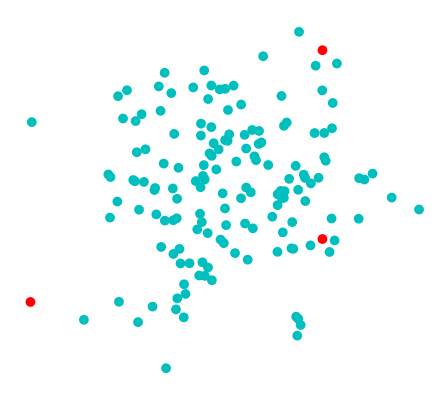
\includegraphics[width=.3\textwidth]{myplot3_1.png}
  %\caption{fig1}
  }
  \quad
  \subfigure[]{
  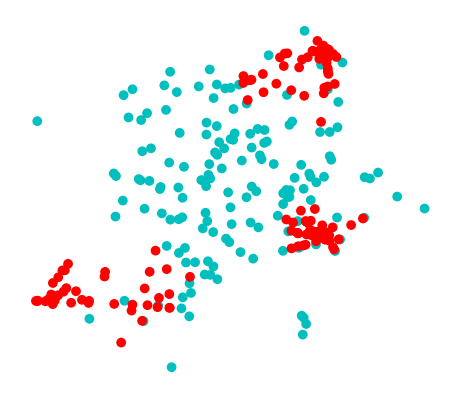
\includegraphics[width=.3\textwidth]{myplot3_2.png}
  }
  \caption{(a) and (b) are distribution of original data and distribution of oversampled data.
  Minority samples in the dataset are too rare and far apart to form effective cluster. 
  We use SMOTE to generate new points.}
  \label{fig14}
  \end{figure}

As shown in Figure\ref{fig14},\ref{fig14}(a) and \ref{fig14}(b) are distribution of original data and distribution
 of oversampled data.
Minority samples in the dataset are too rare and far apart to form effective cluster, we cannot use
gaussian distribution to generate new points, we use SMOTE instead.
Algorithm $generate\_noise$ \ref{alg5} is used to generate new sample points near the noise point.

\subsubsection{Translation of majority points}
new samples are generated according to the distribution characteristics of minority points. 
At the same time we also clean the majority points near minority
points to alleviate the overlapping data distributions.
We use a similar approach to the model CCR\cite{2017CCR}.
When dealing with borderline points, 
the K nearest neighbors of each minority sample is calculated. 
With this sample point as the center and the maximum distance in the K neighbors as the radius, 
a spherical region is drawn. We can move the majority points in these K neighbors out of this region.

\begin{figure}[htbp]
  \centering
  \subfigure[Original]{
  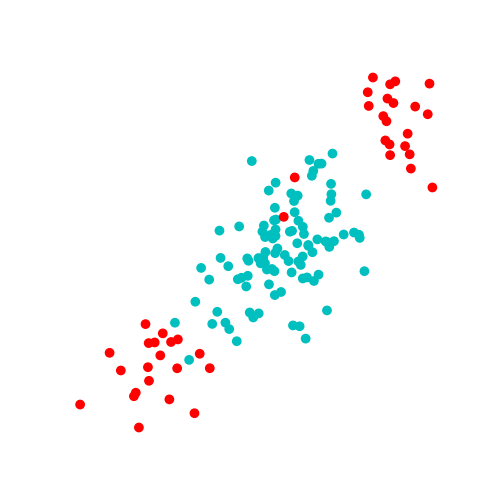
\includegraphics[width=.2\textwidth]{myplot20_0.png}
  %\caption{fig1}
  }
  \quad
  \subfigure[SMOTE]{
  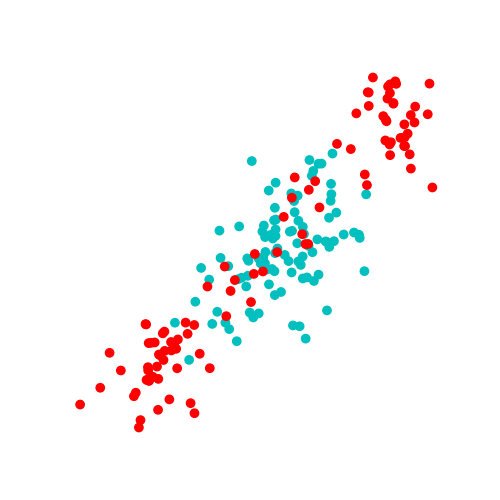
\includegraphics[width=.2\textwidth]{myplot20_1.png}
  }
  \quad
  \subfigure[CCR]{
  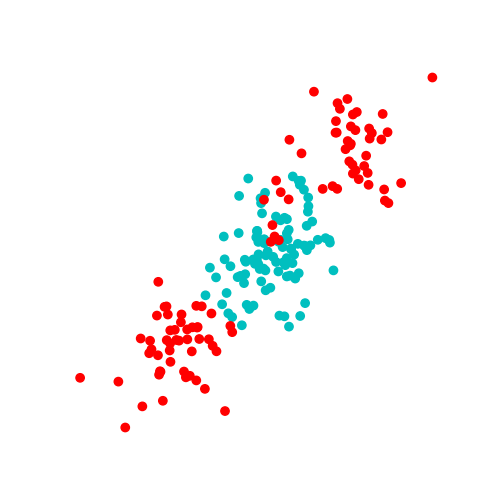
\includegraphics[width=.2\textwidth]{myplot20_2.png}
  }
  \quad
  \subfigure[ODG]{
    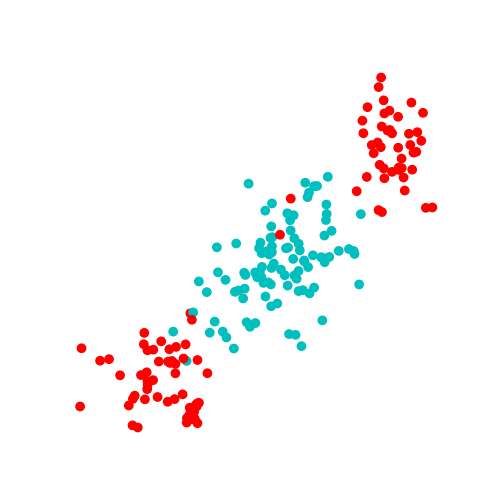
\includegraphics[width=.2\textwidth]{myplot20_3.png}
    }
  \caption{(a) is Original dataset。
  (b),(c),(d) are the oversampling results of SMOTE, CCR and ODG.}
  \label{fig18}
  \end{figure}
We compare the result of SMOTE, CCR and ODG. We assume that some noise points exist in the original data set, 
as well as  clustered minority points. The result shows in Figure\ref{fig18}. 
We can find that after SMOTE, there are overlapping regions, many generated minority points 
overlap with majority points.
Although CCR algorithm avoided overlapping, 
but some minority points were synthesized near the noise, which may produce some interference to predicting results.

\subsubsection{Computational complexity analysis}
We present the time complexity of the oversampling method ODG.
We define the number of majority points is $N_{maj}$, 
the number of minority points is $N_{min}$, the total number of samples is $N$, 
and the number of attributes on the dataset is $m$.
In the DBSCAN algorithm, the time complexity can be controlled at $O(mN_{min}\log(N_{min})$.
which can be simplied to $O(mNlog(N))$.
When calculating the K nearest neighbors of minority points,
The distance between sample points needs to be calculated and sorted, and the complexity of this step is
$O(mN_{min}N+N_{min}Nlog(N))$, it can be simplied as $O(mN^2)$. Therefore the time complexity of
ODG is $O(mN(N+log(N)))$.


\subsection{Multiple classification problem}
\begin{figure}[htbp]
  \centering
  \subfigure[Original dataset]{
  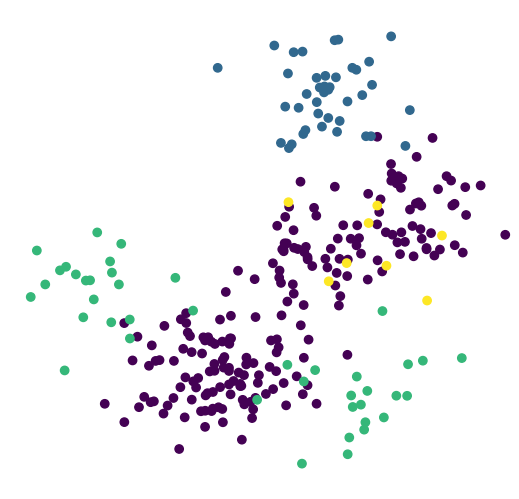
\includegraphics[width=.23\textwidth]{myplot7_1.png}
  %\caption{fig1}
  }
  \quad
  \subfigure[$SMOTE$]{
  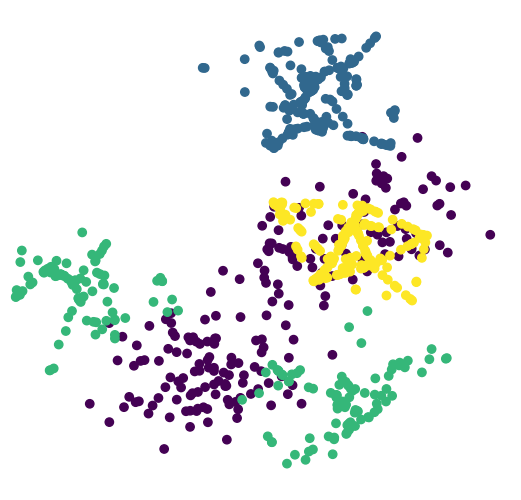
\includegraphics[width=.23\textwidth]{myplot7_2.png}
  }
  \quad
  \subfigure[$Borderline-SMOTE$]{
  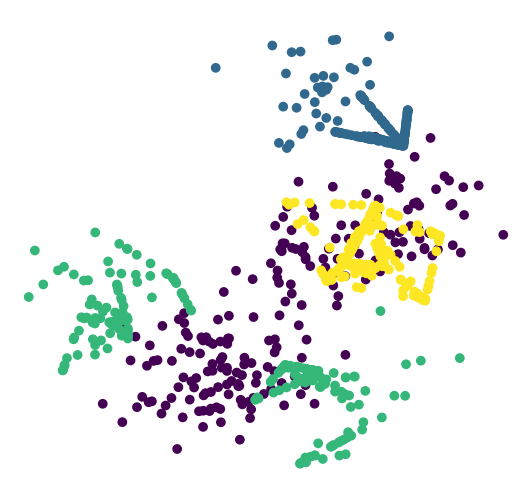
\includegraphics[width=.23\textwidth]{myplot7_3.png}
  }

  \quad
  \subfigure[$SMOTE+ENN$]{
  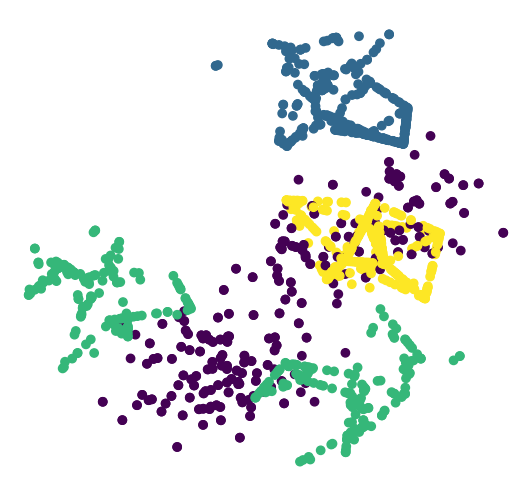
\includegraphics[width=.23\textwidth]{myplot7_4.png}
  }
  \quad
  \subfigure[$MC-ODG$]{
  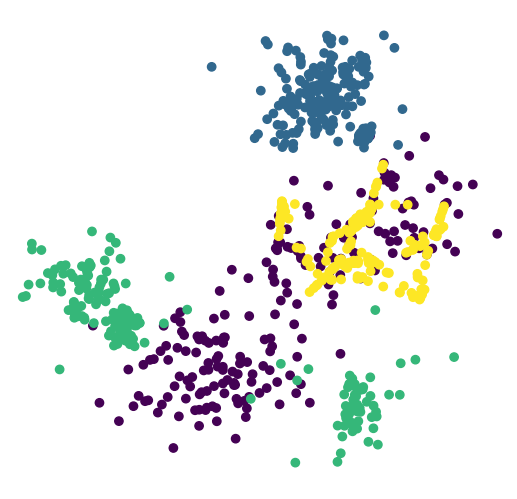
\includegraphics[width=.23\textwidth]{myplot7_5.png}
  }
  \caption{(a) is Original dataset。(b)(c)(d)(e) are oversampling result of SMOTE, 
  Borderline-SMOTE, SMOTE+ENN and MC-ODG.}
  \label{fig17}
  \end{figure}

Multiclassification on imbalance dataset is more difficult to solve than that of binary problem. 
In the binary classification, it is easy to distinguish the majority class and the minority class. 
However, in the multi-classification problem, the relationship between classes is more complex and difficult to deal with.
It is possible to have multiple majority classes or minority classes.
A single class can act as a majority towards some classes, a minority towards others.
In addition, overlapping and noise problems will be more serious.
%The existing approaches to multiclassification can be broadly divided into OVA and OVO\cite{articlemulti},
%We assume that there are m classes, and the OVA problem transforms the multiple 
%classification problem into m binary poblems,
%each taking one as a class separately and leaving the remaining classes as another.
%OVO requires training $m(M-1)/2$ binary classifiers, with one classifier trained between two classes.
%There are problems with both methods.
%The OVA method ignores the information between classes that are merged into a unified class,
%With the increase of the number of categories, the complexity of the OVO method increases rapidly.
The traditional OVA and OVO methods have their own disadvantages, 
\cite{2020Combined,2019Radial} presents a method to deal with multiple classification problems.
We iterate over multiple classes. When we oversample each class,
A subset is selected as a majority class from the already processed classes, 
and the class is treated as a minority class by oversampling methods.
We first sort the classes in reverse order according to the number of samples, and for each minority class, 
from the ones that have been processed,
select a subset of the majority classes, and mark the minority class as the majority
 class after processing the ODG algorithm.
 The overall flow of the MC-ODG algorithm is shown in the algorithm\ref{alg2}.
 \begin{algorithm}[htbp]
  \caption{MC-ODG} %算法的名字
  \label{alg2}
  \hspace*{0.02in} {\bf Input:} %算法的输入, \hspace*{0.02in}用来控制位置,同时利用 \\ 进行换行
   $X$ $\leftarrow$ a data matrix,which has multiple different labels.  \\
   $C$ $\leftarrow$ different classes
  \hspace*{0.02in} {\bf Output:} %算法的结果输出
   $X$ $\leftarrow$ A new data matrix which has been translated and oversamped.
  \begin{algorithmic}[1]
   
  \For{$i \leftarrow 1$ to $|C|$} % For 语句,需要和EndFor对应
    \State $n_{classes}$ $\leftarrow$ number of classes with higher number of points than $C_i$ 
    \If{$n_{classes}$>0}
        \State $X_{min} \leftarrow X^{C_i}$ 
        \State $X_{maj} \leftarrow \emptyset$
        \For{$j \leftarrow 1$ to $n_{classes}$}
            \State add $\lfloor \frac{|X^{C_1}|}{n_{classes}} \rfloor$ randomly chosen points from $X^{(j)}$ to $X_{maj}$
        \EndFor
        \State $X_{maj}^{'},S=ODG(X_{maj},X_{min})$
        \State $X^{C_i} \leftarrow X^{C_i} \cup S$
        \State substitute points used to construct $X_{maj}$ with $X_{maj}^{'}$. 
      \EndIf
  \EndFor
  \State \Return X
  \end{algorithmic}
  \end{algorithm}

 Figure\ref{fig17} shows the original dataset and the oversampling results of SMOTE, Borderline-SMOTE,
 SMOTE+ENN, MC-ODG. We can find that the original data distributions 
 can be retained after oversampling using the $MC-ODG$ algorithm.

 \subsubsection{Computational complexity analysis}
We calculate the time complexity if MC-ODG.
 We also define the total number of samples is N, and the number of attributes on the dataset is $m$.
 The number of classes is $c$. The entire MC-ODG process is equivalent to c-1 times $ODG$.
 Therefore the time complexity of MC-ODG is $O(cmN(N+log(N)))$.

\section{Experiments}
In this section, we will detail a series of experiments on ODG and MC-ODG.
We compared the ODG, MC-ODG algorithms with the existing oversampling methods,
We found that our algorithm ODG and MC-ODG can achieve better results on different metrics.
We also compared the influence of changing the ratio generated near borderline points
on predicting results.
We published the code of our model on github\footnote{https://github.com/Xiaoctw/MC-ODG}.

\subsection{Evaluation matrics}

We evaluated different oversampling methods using multiple metrics. 
Prediction accuracy is not a good metric on imbalanced problems.
Due to the imbalance of data, the accuracy will naturally incline to the majority class.
The predictive ability of the model for minority classes cannot be reflected by accuracy.

\subsubsection{Binary classification}
We labeled the majority class as 0(Negative) and the minority class as 1(Positive).
Precision, Recall, F-value and Auc are more reasonable metrics.
Table\ref{table1} gives the confusion matrix for the binary classification problems.
\begin{table}[htbp]
  \caption{Confusion matrix for the two-class problem}
  \label{table1}
  \centering
  \begin{tabular}{@{}ccc@{}}
  \toprule
  Actual label & \multicolumn{1}{l}{Predicted positive} & \multicolumn{1}{l}{Predicted negative} \\ \midrule
  Positive     & TP                                     & FP                                     \\
  Negative     & FP                                     & FN                                     \\ \bottomrule
  \end{tabular}
  \end{table}
  Using the confusion matrix, 
  we can calculate the Precision, Recall and F-value. The calculation formulas are as follows:
  \begin{equation}
    Precision=\frac{TP}{TP+FP}
  \end{equation}
  \begin{equation}
    Recall=\frac{TP}{TP+FN}
  \end{equation}
  \begin{equation}
    F-value=\frac{(1+\beta^2) \times Precision \times Recall}{\beta^2 \times Precision+Recall}
  \end{equation}

  The value of Auc is defined as the area bounded by the curve of $roc$ and the coordinate axis.
In general, the value of Auc is greater than 0.5. 
The closer the value is to 1, the better the prediction result is.

\subsubsection{Multiple classification}
The evaluation of multi-classification is more complex,
 and there is not a unified evaluation standard and it is still an open problem.
 In addition to the above mentioned Precision, Recall and F-value,
 mGM\ref{equation12} and CBA\ref{equation13} are also introduced in \cite{2017Relevance}.
 \begin{equation}
  \label{equation12}
  CBA=\frac{\sum_{i=1}^{M}\frac{mat_{i,j}}{max(\sum_{j=1}^Mmat_{i,j},\sum_{j=1}^M mat_{j,i})}}{M}
\end{equation}

\begin{equation}
  \label{equation13}
  mGM=\sqrt[M]{\Pi_{i=1}^M Recall_{i}}
\end{equation}

\subsection{Dataset}
The dataset used in the experiment is the classification 
datasets on UCI\footnote{http://archive.ics.uci.edu/ml/datasets.php},
datasets' details are in tables \ref{table3} and \ref{table2}.

\begin{table}[htbp]
  \caption{binary classification dataset}
  \centering
  \label{table3}
  \begin{tabular}{@{}ccccc@{}}
  \toprule
  Datasets                & \multicolumn{1}{l}{Instances} & \multicolumn{1}{l}{Features} & Class distribution & IR  \\ \midrule
  Transfusion(TR)         & 748                           & 5                            & 570/178            & 3.2 \\
  Wisconsin(WIS)           & 699                           & 25                           & 458/241            & 1.9 \\
  Adult(AD)               & 32561                         & 108                          & 24720/7841         & 3.2 \\
  Haberman(HA)            & 336                           & 3                            & 225/81             & 2.8 \\ \bottomrule
  \end{tabular}
  \end{table}
\begin{table}[htbp]
  \caption{multiple classification dataset}
  \centering
  \label{table2}
  \begin{tabular}{@{}cccccc@{}}
  \toprule
  Datasets      & \multicolumn{1}{l}{Instances} & \multicolumn{1}{l}{Features} & \multicolumn{1}{l}{Classes} & Class distribution               & IR  \\ \midrule
  Glass(GL)     & 213                           & 8                            & 6                           & 76/69/29/17/13/9                 & 8.4 \\
  Automobile(AU)& 159                           & 25                           & 6                           & 48/46/29/13/3                    & 16  \\
  Wine(WI)      & 157                           & 12                           & 3                           & 71/58/48                         & 1.5 \\
  Yeast(YE)     & 1484                          & 7                            & 10                          & 463/429/244/163/51/44/35/30/20/4 & 115.6 \\
  Ecoli(EC)     & 336                           & 6                            & 8                           & 143/77/52/35/20/5/2/2 & 71  \\ \bottomrule
  \end{tabular}
  \end{table}

  \begin{table}[htbp]
    \caption{The parameters of ODG and MC-ODG}
    \centering
    \label{table6}
    \setlength{\tabcolsep}{7mm}{
    \begin{tabular}{@{}cc@{}}
    \toprule
    Parameters             & default value \\ \midrule
    k                      & 5             \\
    eps                    & 0.08          \\
    min\_pts               & 4             \\
    fit\_borderline\_ratio & true          \\
    borderline\_ratio      & 0.6           \\
    noise\_ratio           & 0.1           \\
    multiple\_k            & 4             \\ \bottomrule
    \end{tabular}}
  \end{table}
\subsection{Experiment contents}
\subsubsection{Compare the prediction results of different oversampling models}
In this experiment, three widely used machine learning models, C4.5 and K nearest neighbors, and logistic regression were used.
We compared different oversampling methods, SMOTE, Borderline-SMOTE, ADASYN, SMOTE+ENN, MC-CCR and ODG or MC-ODG.
we adopted the cross validation method of K folding, set K=5, repeated the experiment for 10 times, and took the mean value as the final result.
Parameters of ODG and MC-ODG are shown in table \ref{table6}.
$fit\_borderline\_ratio$ means being adaptive to determine the $borderline\_ratio$ or not.
Parameter settings of the other models are shown in table \ref{table4}
\begin{table}[htbp]
    \caption{Parameters}
    \label{table4}
    \centering
    \setlength{\tabcolsep}{7mm}{
    \begin{tabular}{@{}cc@{}}
    \toprule
    Algorithm                            & \multicolumn{1}{l}{Parameters}                                                                                                                                     \\ \midrule
    KNN                                 & k$\in${[}3,5,7{]}                                                                                                                                                  \\
    C4.5                                 & \begin{tabular}[c]{@{}c@{}}max\_depth=5\\ min\_samples\_split=3\end{tabular}                                                                                       \\ \midrule
    MC-CCR                               & \begin{tabular}[c]{@{}c@{}}$energy \in [0.25,0.5,1]$\\ cleaning strategy:translation\\ selection strategy: proportional\\ multi-class decomposition method:sampling\end{tabular} \\
    SMOTE                                & k\_neighbors $\in$ {[}3,5,7{]}                                                                                                                                     \\
    \multicolumn{1}{l}{Borderline-SMOTE} & \begin{tabular}[c]{@{}c@{}}kind="borderline-1"\\ k\_neighbors$\in${[}3,5,7{]}\end{tabular}                                                                         \\
    ADASYN                               & n\_neighbors$\in ${[}3,5,7{]}                                                                                                                                      \\
    \multicolumn{1}{l}{SMOTE+ENN}        & k\_neighbors $\in$ {[}3,5,7{]}                                                                                                                                 \\ \bottomrule
    \end{tabular}}
\end{table}

In ODG and MC-ODG algorithms, DBSCAN algorithm is used for clustering. 
The parameters DBSCAN needs to determine are EPS and min\_pts.
$borderline\_ratio$ of some datasets is artificially specified.
Parameter settings on different datasets are shown in table \ref{table5}.
\begin{table}[htbp]
  \caption{Parameters of ODG, MC-ODG}
  \label{table5}
   \centering
   %\resizebox{\textwidth}{}{
  \begin{tabular}{@{}cc@{}}
  \toprule
  Datasets                & Parameters                                                                                            \\ \midrule
   TR                     & \begin{tabular}[c]{@{}c@{}}eps=0.15\\ min\_pts=3\\ borderline\_ratio=0.5\end{tabular}                    \\
   WIS                    & \begin{tabular}[c]{@{}c@{}}eps=0.5\\ min\_pts=3\\ borderline\_ratio=0.7\end{tabular}                     \\
   AD                     & \begin{tabular}[c]{@{}c@{}}eps=1.6\\ min\_pts=5\\ borderline\_ratio=0.7\end{tabular}                     \\
   HA                     & \begin{tabular}[c]{@{}c@{}}eps=0.14\\ min\_pts=3\end{tabular}                                         \\ \midrule
   GL                     & \begin{tabular}[c]{@{}c@{}}eps=0.15\\ min\_pts=3\end{tabular}                                         \\
   AU                     & \begin{tabular}[c]{@{}c@{}}eps=1.8\\ min\_pts=3\\ borderline\_ratio=0.4\\ noise\_ratio=0.2\end{tabular}  \\
   WI                     & \begin{tabular}[c]{@{}c@{}}eps=0.36\\ min\_pts=2\end{tabular}                                         \\
   EC                     & \begin{tabular}[c]{@{}c@{}}eps=0.14\\ min\_pts=3\\ borderline\_ratio=0.7\end{tabular}                      \\
   YE                     & \begin{tabular}[c]{@{}c@{}}eps=0.13\\ min\_pts=3\\ borderline\_ratio=0.2\\ noise\_ratio=0.9\end{tabular} \\ \bottomrule
  \end{tabular}
  \end{table}

\subsubsection{The effect of $borderline\_ratio$ on the experimental results}
In order to improve the prediction ability of our model,
more minority points need to be generated near the borderline points. 
The parameter $borderline\_ratio$
plays a crucial role.
We choose dataset TR, WIS, AU and EC,
and used matrics F1-score, Auc and mGM to observe the effect of $borderline\_ratio$
on experiment results. We did the experiment five times and took the average.


\subsection{Experiment results}
\subsubsection{Compare the prediction results of different oversampling models}
We give a comparison of different oversampling methods on different 
datasets based on different machine learning models.
For binary datasets, KNN, C4.5 and LR results on multiple metrics are shown in table\ref{table7}, table \ref{table8}, table \ref{table9} 
For multiclassification datasets, KNN, C4.5 and LR results in table \ref{table10}, table \ref{table11} and table \ref{table12}.

\begin{table}[htbp]
  \caption{KNN model deals with binary classification datasets}
  \label{table7}
  \resizebox{\textwidth}{15mm}{
    \begin{tabular}{@{}ccccccccccccccccc@{}}
      \toprule
      \multicolumn{1}{c|}{\multirow{2}{*}{Datasets}}  & \multicolumn{4}{c|}{Precision}                                                                                                               & \multicolumn{4}{c}{Recall}                                                                                                                   & \multicolumn{4}{c|}{F1-score}                                                                                                                & \multicolumn{4}{c}{Auc}                                                                                                               \\ \cmidrule(l){2-17} 
      \multicolumn{1}{c|}{}                           & \multicolumn{1}{c|}{TR}          & \multicolumn{1}{c|}{WIS}                     & \multicolumn{1}{c|}{AD}    & \multicolumn{1}{c|}{HA}       & \multicolumn{1}{c|}{TR}          & \multicolumn{1}{c|}{WIS}                     & \multicolumn{1}{c|}{AD}    & \multicolumn{1}{c|}{HA}       & \multicolumn{1}{c|}{TR}          & \multicolumn{1}{c|}{WIS}                     & \multicolumn{1}{c|}{AD}    & \multicolumn{1}{c|}{HA}       & \multicolumn{1}{c|}{TR}          & \multicolumn{1}{c|}{WIS}                     & \multicolumn{1}{c|}{AD}    & \multicolumn{1}{c}{HA}        \\ \midrule
      None                                            & 0.823                            & 0.934                                        & 0.823                      & 0.426                         & 0.646                            & 0.921                                        & 0.839                      & 0.282                         & 0.717                            & 0.926                                        & 0.83                       & 0.332                         & 0.837                            & 0.955                                        & 0.913                      & 0.604                         \\
      SMOTE                                           & 0.843                            & 0.926                                        & 0.819                      & 0.465                         & 0.604                            & 0.935                                        & 0.837                      & 0.337                         & 0.7                              & 0.93                                         & 0.827                      & 0.381                         & 0.824                            & 0.954                                        & 0.912                      & 0.617                         \\
      Borderline-SMOTE                                & 0.853                            & 0.93                                         & 0.824                      & 0.421                         & 0.606                            & 0.91                                         & 0.839                      & 0.269                         & 0.706                            & 0.919                                        & 0.83                       & 0.319                         & 0.827                            & 0.949                                        & 0.912                      & 0.621                         \\
      ADASYN                                          & \textbf{0.873}                   & \textbf{0.937}                               & 0.819                      & \textbf{0.452}                & 0.618                            & 0.912                                        & 0.843                      & 0.36                          & \textbf{0.721}                   & 0.924                                        & 0.829                      & 0.383                         & 0.834                            & 0.95                                         & 0.913                      & 0.619                         \\
      SMOTE+ENN                                       & 0.71                             & 0.921                                        & 0.797                      & 0.412                         & 0.677                            & 0.953                                        & 0.876                      & 0.537                         & 0.69                             & 0.936                                        & 0.831                      & 0.46                          & 0.806                            & 0.958                                        & 0.912                      & 0.64                          \\
      CCR                                             & 0.738                            & 0.925                                        & 0.794                      & 0.368                         & \textbf{0.808}                   & 0.94                                         & 0.862                      & \textbf{0.626}                & 0.709                            & 0.931                                        & 0.825                      & 0.457                         & 0.834                            & 0.958                                        & 0.909                      & 0.622                         \\
      ODG                                             & 0.8                              & 0.921                                        & \textbf{0.831}             & \textbf{0.452}                & 0.75                             & \textbf{0.956}                               & \textbf{0.879}             & 0.517                         & 0.711                            & \textbf{0.938}                               & \textbf{0.84}              & \textbf{0.476}                & \textbf{0.846}                   & \textbf{0.965}                               & \textbf{0.916}             & \textbf{0.667}                \\ \bottomrule
      \end{tabular}
      }
  \end{table}

\begin{table}[htbp]
    \caption{C4.5 model deals with binary classification datasets}
    \label{table8}
    \resizebox{\textwidth}{15mm}{
      \begin{tabular}{@{}ccccccccccccccccc@{}}
        \toprule
        \multicolumn{1}{c|}{\multirow{2}{*}{Datasets}}  & \multicolumn{4}{c|}{Precision}                                                                                                               & \multicolumn{4}{c}{Recall}                                                                                                                   & \multicolumn{4}{c|}{F1-score}                                                                                                                & \multicolumn{4}{c}{Auc}                                                                                                               \\ \cmidrule(l){2-17} 
        \multicolumn{1}{c|}{}                           & \multicolumn{1}{c|}{TR}          & \multicolumn{1}{c|}{WIS}                     & \multicolumn{1}{c|}{AD}    & \multicolumn{1}{c|}{HA}       & \multicolumn{1}{c|}{TR}          & \multicolumn{1}{c|}{WIS}                     & \multicolumn{1}{c|}{AD}    & \multicolumn{1}{c|}{HA}       & \multicolumn{1}{c|}{TR}          & \multicolumn{1}{c|}{WIS}                     & \multicolumn{1}{c|}{AD}    & \multicolumn{1}{c|}{HA}       & \multicolumn{1}{c|}{TR}          & \multicolumn{1}{c|}{WIS}                     & \multicolumn{1}{c|}{AD}    & \multicolumn{1}{c}{HA}        \\ \midrule
        None                                            & 0.841                            & 0.936                                        & 0.819                      & 0.419                         & 0.6                              & 0.918                                        & 0.848                      & 0.305                         & 0.697                            & 0.926                                        & 0.832                      & 0.34                          & 0.823                            & 0.959                                        & 0.926                      & 0.623                         \\
        SMOTE                                           & \textbf{0.844}                   & 0.93                                         & 0.823                      & 0.448                         & 0.625                            & 0.923                                        & 0.845                      & 0.316                         & \textbf{0.714}                   & 0.935                                        & 0.832                      & 0.359                         & 0.835                            & 0.957                                        & 0.923                      & 0.605                         \\
        Borderline-SMOTE                                & 0.839                            & 0.931                                        & 0.812                      & \textbf{0.482}                & 0.587                            & 0.922                                        & 0.852                      & 0.315                         & 0.684                            & 0.925                                        & 0.83                       & 0.373                         & 0.816                            & 0.958                                        & 0.924                      & 0.594                         \\
        ADASYN                                          & 0.843                            & 0.928                                        & 0.815                      & 0.475                         & 0.596                            & 0.924                                        & 0.848                      & 0.338                         & 0.694                            & 0.924                                        & 0.83                       & 0.388                         & 0.822                            & 0.957                                        & 0.924                      & 0.627                         \\
        SMOTE+ENN                                       & 0.697                            & 0.919                                        & 0.789                      & 0.41                          & 0.673                            & 0.954                                        & \textbf{0.882}             & 0.552                         & 0.678                            & 0.936                                        & 0.834                      & 0.449                         & 0.799                            & 0.959                                        & 0.927                      & 0.628                         \\
        CCR                                             & 0.751                            & 0.918                                        & 0.79                       & 0.367                         & \textbf{0.809}                   & \textbf{0.954}                               & 0.88                       & \textbf{0.628}                & 0.688                            & 0.935                                        & 0.832                      & \textbf{0.465}                & 0.836                            & 0.965                                        & 0.924                      & 0.635                         \\
        ODG                                             & 0.755                            & \textbf{0.938}                               & \textbf{0.824}             & 0.429                         & 0.681                            & 0.951                                        & 0.859                      & 0.524                         & 0.672                            & \textbf{0.943}                               & \textbf{0.84}              & 0.455                         & \textbf{0.843}                   & \textbf{0.968}                               & \textbf{0.928}             & \textbf{0.656}                \\ \bottomrule
        \end{tabular}
        }
\end{table}

\begin{table}[htbp]
      \caption{LR model deals with binary classification datasets}
      \label{table9}
      \resizebox{\textwidth}{15mm}{
        \begin{tabular}{@{}ccccccccccccccccc@{}}
          \hline
          \multicolumn{1}{c|}{\multirow{2}{*}{Datasets}}  & \multicolumn{4}{c|}{Precision}                                                                                                               & \multicolumn{4}{c|}{Recall}                                                                                                                  & \multicolumn{4}{c|}{F1-score}                                                                                                                & \multicolumn{4}{c}{Auc}                                                                                                              \\ \cmidrule(l){2-17} 
          \multicolumn{1}{c|}{}                           & \multicolumn{1}{c|}{TR}          & \multicolumn{1}{c|}{WIS}                     & \multicolumn{1}{c|}{AD}    & \multicolumn{1}{c|}{HA}       & \multicolumn{1}{c|}{TR}          & \multicolumn{1}{c|}{WIS}                     & \multicolumn{1}{c|}{AD}    & \multicolumn{1}{c|}{HA}       & \multicolumn{1}{c|}{TR}          & \multicolumn{1}{c|}{WIS}                     & \multicolumn{1}{c|}{AD}    & \multicolumn{1}{c|}{HA}       & \multicolumn{1}{c|}{TR}          & \multicolumn{1}{c|}{WIS}                     & \multicolumn{1}{c|}{AD}    & \multicolumn{1}{c}{HA}        \\ \midrule
          None                                            & 0.872                            & \textbf{0.962}                               & 0.848                      & \textbf{0.691}                & 0.571                            & 0.946                                        & 0.84                       & 0.284                         & 0.568                            & 0.953                                        & 0.832                      & 0.261                         & 0.847                            & \textbf{0.996}                               & 0.952                      & 0.663                         \\
          SMOTE                                           & 0.892                            & \textbf{0.962}                               & 0.843                      & 0.673                         & 0.549                            & 0.941                                        & 0.82                       & 0.322                         & 0.536                            & 0.951                                        & 0.829                      & 0.309                         & 0.848                            & 0.995                                        & 0.96                       & 0.642                         \\
          Borderline-SMOTE                                & 0.871                            & 0.961                                        & \textbf{0.857}             & 0.653                         & 0.553                            & 0.946                                        & 0.824                      & 0.286                         & 0.549                            & 0.953                                        & 0.837                      & 0.313                         & 0.845                            & 0.992                                        & 0.961                      & 0.663                         \\
          ADASYN                                          & \textbf{0.921}                   & 0.958                                        & 0.852                      & 0.658                         & 0.553                            & 0.95                                         & 0.828                      & 0.321                         & 0.646                            & 0.953                                        & \textbf{0.839}             & 0.309                         & 0.847                            & 0.995                                        & 0.96                       & 0.644                         \\
          SMOTE+ENN                                       & 0.779                            & 0.951                                        & 0.775                      & 0.536                         & 0.701                            & 0.962                                        & 0.895                      & \textbf{0.569}                & 0.663                            & 0.956                                        & \textbf{0.839}             & 0.443                         & 0.847                            & \textbf{0.996}                               & 0.957                      & 0.658                         \\
          CCR                                             & 0.69                             & 0.951                                        & 0.779                      & 0.525                         & 0.763                            & 0.967                                        & 0.884                      & 0.445                         & \textbf{0.665}                   & 0.958                                        & 0.832                      & 0.396                         & 0.848                            & 0.965                                        & 0.957                      & 0.635                         \\
          ODG                                             & 0.655                            & 0.956                                        & 0.775                      & 0.543                         & \textbf{0.781}                   & \textbf{0.968}                               & \textbf{0.906}             & 0.457                         & 0.657                            & \textbf{0.959}                               & 0.834                      & \textbf{0.457}                & \textbf{0.853}                   & \textbf{0.996}                               & \textbf{0.959}             & \textbf{0.668}                \\ \bottomrule
          \end{tabular}
          }
      \end{table}

  % Please add the following required packages to your document preamble:
% \usepackage{multirow}
\begin{table}[htbp]
  \caption{KNN model deals with multi-classification datasets}
  \label{table10}
  \resizebox{\textwidth}{15mm}{
  \begin{tabular}{cccccccccccccccccccccccccc}
  \hline
  \multicolumn{1}{c|}{\multirow{2}{*}{Datasets}}  & \multicolumn{5}{c|}{Precision}                                                                                                                     & \multicolumn{5}{c|}{Recall}                                                                                                                        & \multicolumn{5}{c|}{F1-score}                                                                                                                      & \multicolumn{5}{c|}{mGM}                                                                                                                           & \multicolumn{5}{c}{CBA}                                                                                                                           \\ \cline{2-26} 
  \multicolumn{1}{c|}{}                           & \multicolumn{1}{c|}{AU}         & \multicolumn{1}{c|}{EC}    & \multicolumn{1}{c|}{GL}    & \multicolumn{1}{c|}{WI}   & \multicolumn{1}{c|}{YE}    & \multicolumn{1}{c|}{AU}         & \multicolumn{1}{c|}{EC}    & \multicolumn{1}{c|}{GL}    & \multicolumn{1}{c|}{WI}   & \multicolumn{1}{c|}{YE}    & \multicolumn{1}{c|}{AU}         & \multicolumn{1}{c|}{EC}    & \multicolumn{1}{c|}{GL}    & \multicolumn{1}{c|}{WI}   & \multicolumn{1}{c|}{YE}    & \multicolumn{1}{c|}{AU}         & \multicolumn{1}{c|}{EC}    & \multicolumn{1}{c|}{GL}    & \multicolumn{1}{c|}{WI}   & \multicolumn{1}{c|}{YE}    & \multicolumn{1}{c|}{AU}         & \multicolumn{1}{c|}{EC}    & \multicolumn{1}{c|}{GL}    & \multicolumn{1}{c|}{WI}   & \multicolumn{1}{c}{YE}     \\ \hline
  None                                            & \textbf{0.765}                  & 0.84                       & 0.57                       & 0.962                     & 0.5                        & 0.718                           & 0.78                       & 0.575                      & 0.96                      & 0.492                      & 0.716                           & 0.767                      & 0.555                      & 0.954                     & 0.465                      & 0.713                           & 0.761                      & 0.651                      & 0.958                     & 0.467                      & 0.643                           & 0.717                      & 0.497                      & 0.92                      & 0.419                      \\
  SMOTE                                           & 0.742                           & 0.839                      & 0.572                      & 0.962                     & 0.506                      & 0.695                           & 0.793                      & 0.554                      & 0.969                     & 0.496                      & 0.692                           & 0.802                      & 0.541                      & \textbf{0.963}            & \textbf{0.492}             & 0.643                           & 0.762                      & 0.593                      & \textbf{0.968}            & 0.484                      & 0.618                           & 0.748                      & 0.484                      & 0.931                     & 0.45                       \\
  Borderline-SMOTE                                & 0.716                           & \textbf{0.843}             & 0.578                      & 0.957                     & 0.498                      & 0.677                           & 0.789                      & 0.562                      & 0.963                     & 0.491                      & 0.667                           & 0.802                      & 0.547                      & 0.957                     & 0.486                      & 0.599                           & 0.736                      & 0.633                      & 0.961                     & 0.483                      & 0.591                           & 0.741                      & 0.486                      & 0.924                     & 0.444                      \\
  ADASYN                                          & 0.716                           & \textbf{0.843}             & 0.576                      & 0.955                     & 0.496                      & 0.668                           & 0.793                      & 0.562                      & 0.961                     & 0.494                      & 0.661                           & 0.807                      & 0.547                      & 0.955                     & 0.489                      & 0.621                           & 0.768                      & 0.632                      & 0.959                     & 0.488                      & 0.583                           & 0.756                      & 0.488                      & 0.922                     & 0.449                      \\
  SMOTE+ENN                                       & 0.588                           & 0.823                      & 0.391                      & 0.947                     & \textbf{0.51}              & 0.563                           & 0.815                      & 0.466                      & 0.956                     & 0.485                      & 0.538                           & 0.81                       & 0.401                      & 0.947                     & 0.466                      & 0.481                           & 0.8                        & 0.562                      & 0.953                     & 0.465                      & 0.473                           & \textbf{0.757}             & 0.349                      & 0.903                     & 0.41                       \\
  MC-CCR                                          & 0.719                           & 0.774                      & 0.603                      & 0.955                     & 0.455                      & 0.737                           & 0.803                      & 0.642                      & 0.967                     & 0.5                        & 0.706                           & \textbf{0.811}             & 0.597                      & \textbf{0.963}            & 0.482                      & 0.713                           & 0.775                      & 0.652                      & 0.958                     & \textbf{0.496}             & 0.626                           & 0.717                      & 0.525                      & 0.934                     & 0.445                      \\
  MC-ODG                                          & 0.738                           & 0.805                      & \textbf{0.637}             & \textbf{0.963}            & 0.481                      & \textbf{0.75}                   & \textbf{0.815}             & \textbf{0.664}             & \textbf{0.97}             & \textbf{0.511}             & \textbf{0.721}                  & 0.805                      & \textbf{0.622}             & \textbf{0.963}            & 0.489                      & \textbf{0.725}                  & \textbf{0.803}             & \textbf{0.658}             & 0.967                     & 0.484                      & \textbf{0.641}                  & 0.745                      & \textbf{0.546}             & \textbf{0.935}            & \textbf{0.453}             \\ \hline
  \end{tabular}
  }
\end{table}

\begin{table}[htbp]
    \caption{C4.5 model deals with multi-classification datasets}
    \label{table11}
    \resizebox{\textwidth}{15mm}{
    \begin{tabular}{cccccccccccccccccccccccccc}
    \hline
    \multicolumn{1}{c|}{\multirow{2}{*}{Datasets}}  & \multicolumn{5}{c|}{Precision}                                                                                                                     & \multicolumn{5}{c|}{Recall}                                                                                                                        & \multicolumn{5}{c|}{F1-score}                                                                                                                      & \multicolumn{5}{c|}{mGM}                                                                                                                           & \multicolumn{5}{c}{CBA}                                                                                                                           \\ \cline{2-26} 
    \multicolumn{1}{c|}{}                           & \multicolumn{1}{c|}{AU}         & \multicolumn{1}{c|}{EC}    & \multicolumn{1}{c|}{GL}    & \multicolumn{1}{c|}{WI}   & \multicolumn{1}{c|}{YE}    & \multicolumn{1}{c|}{AU}         & \multicolumn{1}{c|}{EC}    & \multicolumn{1}{c|}{GL}    & \multicolumn{1}{c|}{WI}   & \multicolumn{1}{c|}{YE}    & \multicolumn{1}{c|}{AU}         & \multicolumn{1}{c|}{EC}    & \multicolumn{1}{c|}{GL}    & \multicolumn{1}{c|}{WI}   & \multicolumn{1}{c|}{YE}    & \multicolumn{1}{c|}{AU}         & \multicolumn{1}{c|}{EC}    & \multicolumn{1}{c|}{GL}    & \multicolumn{1}{c|}{WI}   & \multicolumn{1}{c|}{YE}    & \multicolumn{1}{c|}{AU}         & \multicolumn{1}{c|}{EC}    & \multicolumn{1}{c|}{GL}    & \multicolumn{1}{c|}{WI}   & \multicolumn{1}{c}{YE}     \\ \hline
    None                                            & 0.738                           & 0.762                      & 0.658                      & 0.911                     & \textbf{0.541}             & 0.7                             & 0.736                      & 0.63                       & 0.906                     & 0.478                      & 0.695                           & 0.731                      & 0.625                      & 0.904                     & 0.479                      & 0.7                             & 0.723                      & 0.59                       & 0.901                     & 0.574                      & 0.626                           & 0.68                       & 0.567                      & 0.859                     & 0.434                      \\
    SMOTE                                           & 0.702                           & 0.8                        & 0.662                      & 0.934                     & \textbf{0.541}             & 0.685                           & 0.761                      & 0.617                      & 0.918                     & 0.499                      & 0.675                           & 0.768                      & 0.617                      & 0.916                     & 0.5                        & 0.686                           & 0.731                      & 0.639                      & 0.915                     & 0.583                      & 0.614                           & 0.715                      & 0.558                      & 0.873                     & 0.387                      \\
    Borderline-SMOTE                                & 0.741                           & \textbf{0.802}             & 0.67                       & 0.915                     & 0.532                      & 0.718                           & 0.75                       & 0.631                      & 0.908                     & 0.497                      & 0.709                           & 0.759                      & 0.622                      & 0.908                     & 0.498                      & 0.679                           & 0.728                      & 0.594                      & 0.905                     & 0.57                       & 0.642                           & 0.701                      & 0.552                      & 0.869                     & 0.439                      \\
    ADASYN                                          & 0.749                           & 0.789                      & 0.646                      & 0.915                     & 0.539                      & 0.716                           & 0.748                      & 0.619                      & 0.915                     & 0.501                      & 0.708                           & 0.755                      & 0.611                      & 0.912                     & 0.504                      & 0.695                           & 0.739                      & 0.619                      & 0.912                     & 0.576                      & 0.637                           & 0.695                      & 0.543                      & 0.881                     & 0.449                      \\
    SMOTE+ENN                                       & 0.577                           & 0.761                      & 0.45                       & 0.906                     & 0.491                      & 0.564                           & 0.739                      & 0.528                      & 0.907                     & 0.442                      & 0.524                           & 0.726                      & 0.464                      & 0.901                     & 0.443                      & 0.542                           & 0.71                       & \textbf{0.677}             & 0.902                     & 0.523                      & 0.495                           & 0.658                      & 0.411                      & 0.853                     & 0.387                      \\
    MC-CCR                                          & \textbf{0.773}                  & 0.788                      & 0.658                      & 0.923                     & 0.435                      & \textbf{0.748}                  & \textbf{0.788}             & 0.675                      & 0.931                     & 0.492                      & 0.731                           & 0.777                      & 0.638                      & 0.929                     & 0.491                      & 0.73                            & 0.771                      & 0.64                       & 0.928                     & \textbf{0.605}             & 0.666                           & 0.717                      & 0.567                      & 0.891                     & 0.443                      \\
    MC-ODG                                          & 0.762                           & 0.797                      & \textbf{0.684}             & \textbf{0.945}            & 0.501                      & 0.738                           & 0.786                      & \textbf{0.694}             & \textbf{0.944}            & \textbf{0.536}             & \textbf{0.742}                  & \textbf{0.781}             & \textbf{0.663}             & \textbf{0.943}            & \textbf{0.504}             & \textbf{0.749}                  & \textbf{0.773}             & 0.634                      & \textbf{0.943}            & 0.584                      & \textbf{0.676}                  & \textbf{0.726}             & \textbf{0.592}             & \textbf{0.913}            & \textbf{0.45}              \\ \hline
    \end{tabular}
    }
\end{table}


\begin{table}[htbp]
      \caption{LR model deals with multi-classification datasets}
      \label{table12}
      \resizebox{\textwidth}{15mm}{
      \begin{tabular}{cccccccccccccccccccccccccc}
      \hline
      \multicolumn{1}{c|}{\multirow{2}{*}{Datasets}}  & \multicolumn{5}{c|}{Precision}                                                                                                                     & \multicolumn{5}{c|}{Recall}                                                                                                                        & \multicolumn{5}{c|}{F1-score}                                                                                                                      & \multicolumn{5}{c|}{mGM}                                                                                                                           & \multicolumn{5}{c}{CBA}                                                                                                                           \\ \cline{2-26} 
      \multicolumn{1}{c|}{}                           & \multicolumn{1}{c|}{AU}         & \multicolumn{1}{c|}{EC}    & \multicolumn{1}{c|}{GL}    & \multicolumn{1}{c|}{WI}   & \multicolumn{1}{c|}{YE}    & \multicolumn{1}{c|}{AU}         & \multicolumn{1}{c|}{EC}    & \multicolumn{1}{c|}{GL}    & \multicolumn{1}{c|}{WI}   & \multicolumn{1}{c|}{YE}    & \multicolumn{1}{c|}{AU}         & \multicolumn{1}{c|}{EC}    & \multicolumn{1}{c|}{GL}    & \multicolumn{1}{c|}{WI}   & \multicolumn{1}{c|}{YE}    & \multicolumn{1}{c|}{AU}         & \multicolumn{1}{c|}{EC}    & \multicolumn{1}{c|}{GL}    & \multicolumn{1}{c|}{WI}   & \multicolumn{1}{c|}{YE}    & \multicolumn{1}{c|}{AU}         & \multicolumn{1}{c|}{EC}    & \multicolumn{1}{c|}{GL}    & \multicolumn{1}{c|}{WI}   & \multicolumn{1}{c}{YE}     \\ \hline
      None                                            & 0.668                           & 0.657                      & \textbf{0.642}             & 0.984                     & \textbf{0.523}             & 0.62                            & 0.607                      & 0.575                      & 0.98                      & 0.416                      & 0.617                           & 0.679                      & 0.615                      & 0.973                     & 0.423                      & 0.709                           & 0.702                      & 0.583                      & 0.984                     & 0.521                      & 0.594                           & 0.538                      & 0.519                      & 0.963                     & 0.471                      \\
      SMOTE                                           & \textbf{0.741}                  & 0.674                      & 0.622                      & 0.984                     & 0.548                      & 0.676                           & 0.601                      & 0.594                      & 0.985                     & 0.425                      & 0.681                           & 0.675                      & 0.608                      & 0.984                     & 0.436                      & 0.678                           & 0.716                      & 0.584                      & 0.985                     & 0.533                      & 0.618                           & 0.544                      & 0.525                      & 0.969                     & 0.48                       \\
      Borderline-SMOTE                                & 0.733                           & 0.663                      & 0.63                       & 0.985                     & 0.502                      & 0.665                           & 0.605                      & 0.592                      & 0.984                     & 0.411                      & 0.669                           & 0.66                       & 0.618                      & 0.984                     & 0.437                      & 0.629                           & 0.719                      & 0.603                      & 0.984                     & 0.591                      & 0.603                           & 0.548                      & 0.509                      & 0.967                     & 0.472                      \\
      ADASYN                                          & 0.707                           & 0.687                      & 0.626                      & 0.984                     & 0.502                      & 0.636                           & 0.602                      & 0.610                      & 0.984                     & 0.415                      & 0.648                           & 0.656                      & 0.603                      & 0.985                     & 0.44                       & 0.626                           & 0.706                      & 0.610                      & 0.983                     & 0.591                      & 0.592                           & 0.558                      & 0.531                      & 0.971                     & 0.474                      \\
      SMOTE+ENN                                       & 0.57                            & 0.551                      & 0.61                       & 0.965                     & 0.434                      & 0.558                           & 0.543                      & 0.622                      & 0.975                     & 0.41                       & 0.528                           & 0.62                       & 0.605                      & 0.967                     & 0.407                      & 0.537                           & 0.768                      & \textbf{0.679}             & 0.97                      & \textbf{0.67}              & 0.478                           & 0.502                      & 0.506                      & 0.946                     & 0.39                       \\
      MC-CCR                                          & 0.718                           & 0.679                      & 0.624                      & 0.983                     & 0.493                      & 0.711                           & 0.693                      & \textbf{0.673}             & \textbf{0.99}             & 0.515                      & 0.701                           & 0.672                      & 0.63                       & 0.983                     & 0.537                      & 0.691                           & 0.866                      & 0.652                      & 0.985                     & 0.581                      & 0.644                           & 0.628                      & 0.566                      & 0.869                     & 0.517                      \\
      MC-ODG                                          & 0.7                             & 0.723                      & 0.633                      & \textbf{0.988}            & 0.473                      & \textbf{0.74}                   & 0.758                      & 0.659                      & 0.986                     & \textbf{0.52}              & \textbf{0.705}                  & \textbf{0.723}             & \textbf{0.657}             & \textbf{0.989}            & \textbf{0.558}             & \textbf{0.763}                  & \textbf{0.882}             & 0.671                      & \textbf{0.99}             & 0.586                      & \textbf{0.646}                  & \textbf{0.663}             & \textbf{0.577}             & \textbf{0.979}            & \textbf{0.525}             \\ \hline
      \end{tabular}
      }
\end{table}


In the oversampling of binary-classification, 
we found that the ODG algorithm can achieve the best results on multiple metrics of most datasets.
Best results can be obtained because we consider that the data may be distributed in clusters, 
and we adopt different oversampling methods for data points in different positions.
Minority sample data are generated retaining the distribution characteristics of the original data, 
enhancing the ability of machine learning.
It is obvious that the MC-ODG and MC-CCR are superior to other oversampling methods in  
multi-classification tasks. 
The reason is that both approaches take into account the relationships between different classes and
can avoid overlapping data distribution.
Meanwhile, the MC-ODG algorithm is superior to MC-CCR, because MC-ODG
algorithm can retain the original data distribution when generating data.

We also found the following additional conclusions:
\begin{itemize}
  \item Good results can be achieved on the Precision metric without any oversampling progress. 
   the best results can be obtained on the data set WIS without oversampling.
   When we generate large numbers of minority sample points, 
   the model will be inclined to predict the results as minority samples. In this way, 
   the value of TP+FP will become larger, while the value of TP is limited, then the Precision will decrease.
  \item Different datasets have different distribution characteristics
   and are suited to different machine learning methods.
  For example, the LR model on WIS can get good prediction results, while KNN is poor. 
  And on the HA dataset
  The prediction result of KNN algorithm is much better than that of LR algorithm.
  \item Different oversampling methods are suitable for different datasets. 
  Such as CCR method is very suitable for TR, 
  SMOTE+ENN is suitable for AD.
  \item CCR method can obtain good results, 
  the reason is that the CCR method can effectively avoid overlapping and handle noise data.
\end{itemize}


\subsubsection{The effect of $borderline\_ratio$ on the experimental results}
Figure\ref{fig13} shows the influence of the change with $borderline\_ratio$
on the model prediction results.
\ref{fig13}(a),\ref{fig13}(b) represents the change trend of Auc and F1-score on the binary data set. 
\ref{fig13}(c),\ref{fig13}(d) represents the trend of F1-score and mGM on multiclassification datasets. 
It was observed that the variation trend of the predicted results remained the same on different metrics. 
The prediction results are optimal near a certain ratio.
Except for the AU data set, $boaderline\_ratio$ is greater than 0.5 when the best result are obtained. 
It shows that in order to make the machine learning model more inclined to the learning of minority points, 
we need to generate more sample points near the boundary points.
We find that after reaching the peak, as the $borderline\_ratio$ increases,
The rate of decline is slower than the rate of rise before reaching the peak.
This also indicates that the generation of minority sample 
points near the boundary is conducive to enhancing the prediction results.
\begin{figure}[htbp]
  \centering
  \subfigure[]{
  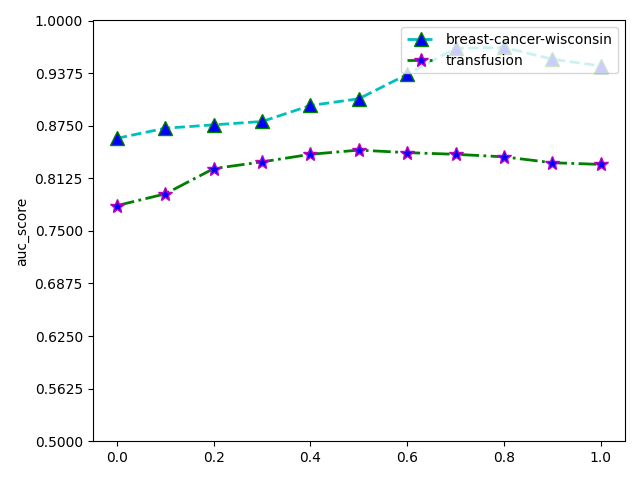
\includegraphics[width=.25\textwidth]{transfusion_breast_auc.png}
  %\caption{fig1}
  }
  \quad
  \subfigure[]{
  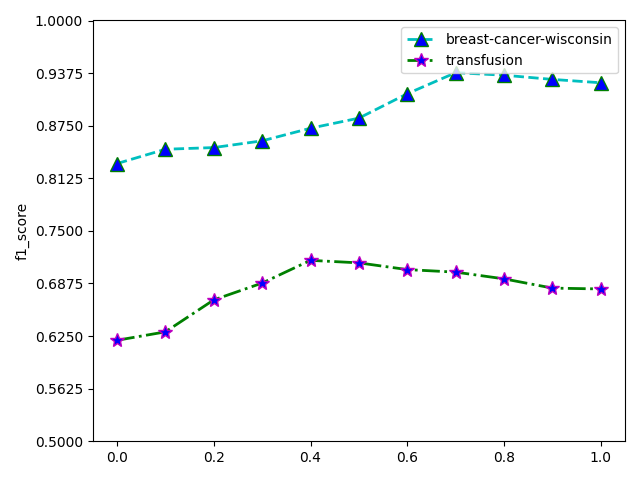
\includegraphics[width=.25\textwidth]{transfusion_breast_f1.png}
  }
  
  \quad
  \subfigure[]{
  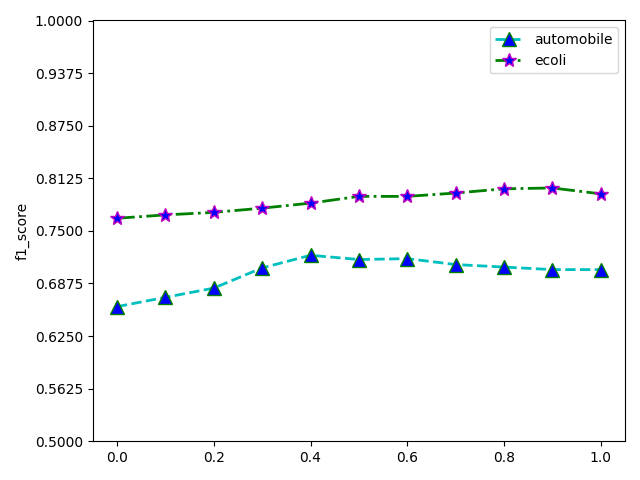
\includegraphics[width=.25\textwidth]{automobile_ecoli_f1.png}
  }
  \quad
  \subfigure[]{
  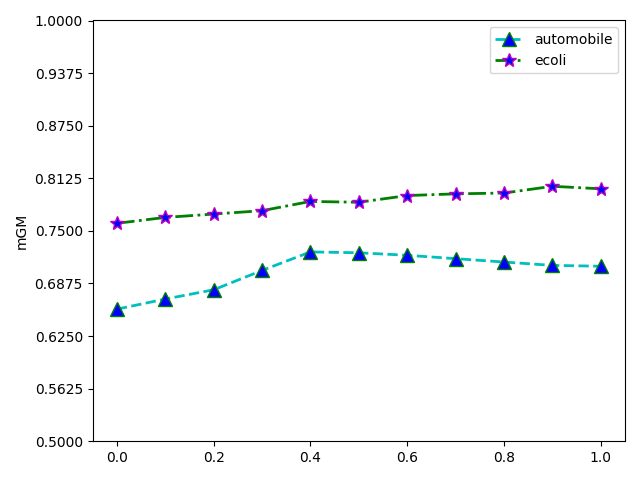
\includegraphics[width=.25\textwidth]{automobile_ecoli_mGM.png}
  }
  \caption{Effect of $borderline\_ratio$ on experiment results}
  \label{fig13}
  \end{figure}


\section{Conclusions and future work}
This paper presents a new oversampling method. 
The ODG algorithm is used to solve the binary classification problem while the MC-ODG algorithm
 is used to solve the multi-classification problem. In the ODG algorithm, 
 we first use the DBSCAN algorithm to cluster minority points and
 get the core points, borderline points and noise points.
 Different oversampling methods are used to deal with different points.
The key is generating new samples near the borderline points.
When new samples are generated, 
the distribution of the generated data depends on the variance of the core points.
The number generated is positively correlated with the number of majority points near the boundary point.
Meanwhile majority samples in the K nearest neighbors 
are moved out of the maximum distance in the K neighbors to avoid overlapping.
MC-ODG takes an iterative approach for each class. 
In each oversampling process, the distribution information of other majority classes is used.
Compared with previous proposed oversampling methods, 
the method to generate data points retains the original data distribution, 
can effectively avoid overlapping and handle noise data points.
Experimental results show that it is an effective method.

In our future work, we will consider how to implement oversampling in a simpler way.
We find that lots of parameters to be processed in ODG and MC-ODG. 
we will consider how to reduce the parameters, which can also achieve relatively good results.
\begin{thebibliography}{8}
  \bibitem{2020EASY}
  Abdullah, S. and Prasetyo, G.~V. (2020).
  \newblock Easy ensemmble with random forest to handle imbalanced data in
    classification.
  
  \bibitem{2007K}
  Arthur, D. and Vassilvitskii, S. (2007).
  \newblock K-means++: The advantages of careful seeding.
  \newblock In {\em Proceedings of the Eighteenth Annual ACM-SIAM Symposium on
    Discrete Algorithms, SODA 2007, New Orleans, Louisiana, USA, January 7-9,
    2007}.
  
  \bibitem{2016A}
  Branco, P., Torgo, L., and Ribeiro, R.~P. (2016).
  \newblock {\em A Survey of Predictive Modeling on Imbalanced Domains}.
  \newblock ACM.
  
  \bibitem{2017Relevance}
  Branco, P., Torgo, L., Ribeiro, R.~P., Branco, P., Torgo, L., Ribeiro, R.~P.,
    Branco, P., Torgo, L., Ribeiro, R.~P., and Branco, P. (2017).
  \newblock {\em Relevance-Based Evaluation Metrics for Multi-class Imbalanced
    Domains}.
  
  \bibitem{2011LIBSVM}
  Chang, C. C. C.~C. and Lin, C. C.~C. (2011).
  \newblock Libsvm: A library for support vector machines.
  
  \bibitem{2004Editorial}
  Chawla, N., Japkowic, N., Kotcz, A., and Japkowicz, N. (2004).
  \newblock Editorial: Special issues on learning from imbalanced data sets.
  \newblock {\em Annals of Nuclear Energy}, 36(3):255--257.
  
  \bibitem{2002SMOTE}
  Chawla, N.~V., Bowyer, K.~W., Hall, L.~O., and Kegelmeyer, W.~P. (2002).
  \newblock Smote: Synthetic minority over-sampling technique.
  \newblock {\em Journal of Artificial Intelligence Research}, 16(1):321--357.
  
  \bibitem{2003SMOTEBoost}
  Chawla, N.~V., Lazarevic, A., Hall, L.~O., and Bowyer, K.~W. (2003).
  \newblock Smoteboost: Improving prediction of the minority class in boosting.
  \newblock In {\em European Conference on Principles of Data Mining and
    Knowledge Discovery}.
  
  \bibitem{Chen_2016}
  Chen, T. and Guestrin, C. (2016).
  \newblock Xgboost.
  \newblock {\em Proceedings of the 22nd ACM SIGKDD International Conference on
    Knowledge Discovery and Data Mining}.
  
  \bibitem{2008DATA}
  David, P.~I., James, G.~R., and Neil, W. (2008).
  \newblock Data distribution system and method.
  
  \bibitem{2018SMOTE}
  Fernandez, A., Garcia, S., Chawla, N.~V., and Herrera, F. (2018).
  \newblock Smote for learning from imbalanced data: Progress and challenges,
    marking the 15-year anniversary.
  \newblock {\em Journal of Artificial Intelligence Research}, 61:863--905.
  
  \bibitem{articlemulti}
  Fernández, A., López, V., Galar, M., Del~Jesus, M.~J., and Herrera, F.
    (2013).
  \newblock Analysing the classification of imbalanced data-sets with multiple
    classes: Binarization techniques and ad-hoc approaches.
  \newblock {\em Knowledge-Based Systems}, 42:97–110.
  
  \bibitem{article_boosting}
  Ferreira, A. and Figueiredo, M. (2012).
  \newblock Boosting algorithms: A review of methods, theory, and applications.
  \newblock {\em Ensemble Machine Learning: Methods and Applications}, 3:35--85.
  
  \bibitem{10.1007/3-540-59119-2_166}
  Freund, Y. and Schapire, R.~E. (1995).
  \newblock A desicion-theoretic generalization of on-line learning and an
    application to boosting.
  \newblock In Vit{\'a}nyi, P., editor, {\em Computational Learning Theory},
    pages 23--37, Berlin, Heidelberg. Springer Berlin Heidelberg.
  
  \bibitem{2005Borderline}
  Han, H., Wang, W., and Mao, B. (2005).
  \newblock Borderline-smote: A new over-sampling method in imbalanced data sets
    learning.
  \newblock In {\em International Conference on Intelligent Computing}.
  
  \bibitem{2008ADASYN}
  He, H., Bai, Y., Garcia, E.~A., and Li, S. (2008).
  \newblock Adasyn: Adaptive synthetic sampling approach for imbalanced learning.
  \newblock In {\em Neural Networks, 2008. IJCNN 2008. (IEEE World Congress on
    Computational Intelligence). IEEE International Joint Conference on}.
  
  \bibitem{Jierui2013Overlapping}
  Jierui, Xie, Stephen, Kelley, Boleslaw, K., and Szymanski (2013).
  \newblock Overlapping community detection in networks: The state-of-the-art and
    comparative study.
  \newblock {\em Acm Computing Surveys}.
  
  \bibitem{2010A}
  Kanimozhi, M.~A. (2010).
  \newblock A multiple resampling method for learning from imbalanced data sets.
  \newblock {\em Computational Intelligence}, 20(1):18--36.
  
  \bibitem{article}
  Kotsiantis, S., Kanellopoulos, D., and Pintelas, P. (2005).
  \newblock Handling imbalanced datasets: A review.
  \newblock {\em GESTS International Transactions on Computer Science and
    Engineering}, 30:25--36.
  
  \bibitem{2020Combined}
  Koziarski, M., Woniak, M., and Krawczyk, B. (2020).
  \newblock Combined cleaning and resampling algorithm for multi-class imbalanced
    data with label noise.
  
  \bibitem{2017CCR}
  Koziarski, M. and Wozniak, M. (2017).
  \newblock Ccr: A combined cleaning and resampling algorithm for imbalanced data
    classification.
  \newblock {\em International Journal of Applied Mathematics and Computer ence},
    27(4):727--736.
  
  \bibitem{2019Radial}
  Krawczyk, B., Koziarski, M., and Wozniak, M. (2019).
  \newblock Radial-based oversampling for multiclass imbalanced data
    classification.
  \newblock {\em IEEE Transactions on Neural Networks and Learning Systems},
    PP(99):1--14.
  
  \bibitem{2018Multi}
  Lango, M. and Stefanowski, J. (2018).
  \newblock Multi-class and feature selection extensions of roughly balanced
    bagging for imbalanced data.
  \newblock {\em Journal of Intelligent Information Systems}, 50(1):97--127.
  
  \bibitem{Victoria2013An}
  López, V., Fernández, A., García, S., Palade, V., and Herrera, F. (2013).
  \newblock An insight into classification with imbalanced data: Empirical
    results and current trends on using data intrinsic characteristics.
  \newblock {\em Information ences}, 250:113--141.
  
  \bibitem{2013Mining}
  Ma, X., Wu, Y.~J., Wang, Y., Chen, F., and Liu, J. (2013).
  \newblock Mining smart card data for transit riders' travel patterns.
  \newblock {\em Transportation Research}, 36C(nov.):1--12.
  
  \bibitem{2007Highcost-sensitive}
  Masnadi-Shirazi, H. and Vasconcelos, N. (2007).
  \newblock High detection-rate cascades for real-time object detection.
  \newblock In {\em Computer Vision, 2007. ICCV 2007. IEEE 11th International
    Conference on}.
  
  \bibitem{2010Risk}
  Masnadi-Shirazi, H. and Vasconcelos, N. (2010).
  \newblock Risk minimization, probability elicitation, and cost-sensitive svms.
  \newblock In {\em International Conference on Machine Learning}.
  
  \bibitem{2004A}
  Monard, M.~C., Monard, M.~C., and Monard, M.~C. (2004).
  \newblock {\em A study of the behavior of several methods for balancing machine
    learning training data}.
  \newblock ACM.
  
  \bibitem{Myoung2015Geometric}
  Myoung-Jong, Kim, Dae-Ki, Kang, Hong, Bae, and Kim (2015).
  \newblock Geometric mean based boosting algorithm with over-sampling to resolve
    data imbalance problem for bankruptcy prediction.
  \newblock {\em Expert Systems with Applications}.
  
  \bibitem{2013Computational}
  Nahar, J., Imam, T., Tickle, K.~S., and Chen, Y. P.~P. (2013).
  \newblock Computational intelligence for heart disease diagnosis: A medical
    knowledge driven approach.
  \newblock {\em Expert Systems with Applications}, 40(1):96--104.
  
  \bibitem{2015Undersampled}
  Peters, D.~C., Korosec, F.~R., Grist, T.~M., Block, W.~F., Holden, J.~E.,
    Vigen, K.~K., and Mistretta, C.~A. (2015).
  \newblock Undersampled projection reconstruction applied to mr angiography.
  \newblock {\em Magnetic Resonance in Medicine}, 43(1):91--101.
  
  \bibitem{2004Minority}
  Phua, C., Alahakoon, D., and Lee, V. (2004).
  \newblock Minority report in fraud detection: Classification of skewed data.
  \newblock {\em Acm Sigkdd Explorations Newsletter}, 6(1):50--59.
  
  \bibitem{2019Class}
  Raghuwanshi, B.~S. and Shukla, S. (2019).
  \newblock Class imbalance learning using underbagging based kernelized extreme
    learning machine.
  \newblock {\em Neurocomputing}, 329(FEB.15):172--187.
  
  \bibitem{inproceedings}
  Sanguanmak, Y. and Hanskunatia, A. (2016).
  \newblock Dbsm: The combination of dbscan and smote for imbalanced data
    classification.
  \newblock pages 1--5.
  
  \bibitem{SEEGER2004GAUSSIAN}
  SEEGER and MATTHIAS (2004).
  \newblock Gaussian processes for machine learning.
  \newblock {\em International Journal of Neural Systems}.
  
  \bibitem{2019Electrocardiogram}
  Sun, L., Shang, Z., Cao, Q., Chen, K., and Li, J. (2019).
  \newblock Electrocardiogram diagnosis based on smote+enn and random forest.
  
  \bibitem{multi_class}
  {Wang}, S. and {Yao}, X. (2012).
  \newblock Multiclass imbalance problems: Analysis and potential solutions.
  \newblock {\em IEEE Transactions on Systems, Man, and Cybernetics, Part B
    (Cybernetics)}, 42(4):1119--1130.
  
  \bibitem{2011Data}
  Witten, I.~H., Frank, E., Hall, M.~A., and Booksx, I. (2011).
  \newblock Data mining: Practical machine learning tools and techniques, third
    edition.
  \newblock {\em Acm Sigmod Record}, 31(1):76--77.
  
  \bibitem{2020Over}
  Xiaolong, X., Wen, C., and Yanfei, S. (2020).
  \newblock Over-sampling algorithm for imbalanced data classification.
  \newblock {\em Journal of Systems Engineering and Electronics},
    30(6):1182--1191.
  
  \bibitem{2007LogitBoost}
  Zhang, G. and Fang, B. (2007).
  \newblock Logitboost classifier for discriminating thermophilic and mesophilic
    proteins.
  \newblock {\em Journal of Biotechnology}, 127(3):417--424.
  
  \bibitem{2018Imbalanced}
  Zhang, Y., Li, X., Gao, L., Wang, L., and Wen, L. (2018).
  \newblock Imbalanced data fault diagnosis of rotating machinery using synthetic
    oversampling and feature learning.
  \newblock {\em Journal of Manufacturing Systems}, 48(Part C):34--50.
\end{thebibliography}
\bibliographystyle{splncs04}
\bibliography{mybibliography1}
%
%\end{document}
\end{document}


